\NeedsTeXFormat{LaTeX2e}
\documentclass[a4paper,
10pt,
headsepline,           % Linie zw. Kopfzeile und Text
twoside,
openright,
pointlessnumbers,      % keine Punkte nach den letzten Ziffern in Überschriften
bibtotoc,              % LV im IV
chapterprefix,
DIV=9,                
%BCOR15mm               % Bindekorrektur
]{scrbook}
\KOMAoptions{DIV=last} % Neuberechnung Satzspiegel nach Laden von Paket helvet

\pagestyle{headings}
\usepackage{blindtext}

% für Texte in deutscher Sprache
\usepackage[ngerman]{babel}
\usepackage[utf8]{inputenc}
\usepackage[T1]{fontenc}

% Helvetica als Standard-Dokumentschrift
\usepackage[scaled]{helvet}
\renewcommand{\familydefault}{\sfdefault} 

% Literaturverzeichnis mit BibLKaTeX
\usepackage[babel,german=quotes]{csquotes}
\usepackage[backend=bibtex8,sorting=none,style=numeric-comp]{biblatex}
\DefineBibliographyStrings{ngerman}{
	andothers = {{et~al.}},
}
\bibliography{bibliography}
\bibliography{Neuroprojekt}
\renewcommand*{\bibfont}{\small}

\usepackage{tikz}
\tikzset{every picture/.style={line width=0.75pt}} 

\usepackage{fix-cm}
\usepackage{titlesec}

\usepackage{graphicx}
\usepackage{tabularx}
\usepackage{booktabs}
\usepackage{longtable}
\usepackage{multirow}
\usepackage{multicol}
\usepackage{float}
\usepackage{subfig}
\usepackage{dblfloatfix}

% Besondere Schriftauszeichnungen
\usepackage{xurl}              % \url{http://...} in Schreibmaschinenschrift
\usepackage{color}            % zum Setzen farbigen Textes
\usepackage{xcolor}
\usepackage{nicefrac}
\usepackage{amssymb, amsmath, amsthm} % Pakete für Mathe-Umgebungen und -Symbole

\definecolor{grayChapt}{gray}{0.65}
\titleformat{\chapter}[display]{\filleft\Huge\bfseries}{\vspace*{-5cm}\fontsize{100}{100}\selectfont\textcolor{grayChapt}\thechapter}{-1.9ex}{}[]%
\titleformat{\section}{\normalfont\Large\bfseries}{\thesection}{1em}{}
\titleformat{\subsection}{\normalfont\large\bfseries}{\thesubsection}{1em}{}

\newtheorem{definition}{Definition}

\usepackage{setspace}         % Paket für div. Abstände, z.B. ZA
\setlength{\parindent}{0pt}   % kein linker Einzug der ersten Absatzzeile
\setlength{\parskip}{1.4ex plus 0.35ex minus 0.3ex} % Absatzabstand, leicht variabel

% Tiefe, bis zu der Überschriften in das Inhaltsverzeichnis kommen
\setcounter{tocdepth}{3}      % ist Standard

% Beispiele für Quellcode
\usepackage{listings}
\definecolor{codegreen}{rgb}{0,0.6,0}
\definecolor{codegray}{rgb}{0.5,0.5,0.5}
\definecolor{codepurple}{rgb}{0.58,0,0.82}
\definecolor{backcolour}{rgb}{0.95,0.95,0.92}
\lstset{
	backgroundcolor=\color{backcolour},   
	commentstyle=\color{codegreen},
	keywordstyle=\color{magenta},
	numberstyle=\tiny\color{codegray},
	stringstyle=\color{codepurple},
	basicstyle=\ttfamily\footnotesize,
	breakatwhitespace=false,         
	breaklines=true,                 
	captionpos=b,                    
	keepspaces=true,                 
	numbers=left,                    
	numbersep=5pt,                  
	showspaces=false,                
	showstringspaces=false,
	showtabs=false,                  
	tabsize=2
}
\renewcommand{\lstlistingname}{Quellcode}

\usepackage{booktabs}

% hier Namen etc. einsetzen
\newcommand{\fullnameA}{Joshua Hirschbrunn}
\newcommand{\emailA}{joshua.hirschbrunn@uni-ulm.de}
\newcommand{\fullnameB}{Jonathan Schilling}
\newcommand{\emailB}{jonathan.schilling@uni-ulm.de}
\newcommand{\fullnameC}{Tim Schneider}
\newcommand{\emailC}{tim-3.schneider@uni-ulm.de}
\newcommand{\fullnameD}{Daniela Tust}
\newcommand{\emailD}{daniela.tust@uni-ulm.de}
\newcommand{\titel}{Generieren und Manipulieren von Bildern mit GANs}
\newcommand{\jahr}{2022}
\newcommand{\matnrA}{980580}%TODO Matrikelnr. Joshua
\newcommand{\matnrB}{980556}
\newcommand{\matnrC}{982435}
\newcommand{\matnrD}{123456}%TODO Matrikelnr. Dani
\newcommand{\gutachterA}{Prof.\,Dr.\,Friedhelm Schwenker}

% hier die Fakultät auswählen
\newcommand{\fakultaet}{Ingenieurwissenschaften, Informatik und Psychologie}
% hier das Institut einsetzen
\newcommand{\institut}{Institut für Neuroinformatik}

% Informationen, die LaTeX in die PDF-Datei schreibt
\pdfinfo{
  /Author (\fullnameA, \fullnameB, \fullnameC, \fullnameD)
  /Title (\titel)
  /Producer     (pdfeTex 3.14159-1.30.6-2.2)
  /Keywords ()
}

\definecolor{dark blue}{HTML}{000066}

\definecolor{todoCite}{HTML}{ABD4B6}%Quellen raussuchen
\definecolor{todoRef}{HTML}{A7C5DB}%Auf glossar, acronyme, bilder etc referenzieren
\definecolor{todoNorm}{HTML}{E6C59E}%Sonstige Todos
\definecolor{todoCont}{HTML}{B483C9}%Inhalte

\usepackage[hyperfootnotes=false]{hyperref}
\usepackage[multiple]{footmisc}
\usepackage[all]{hypcap}
\hypersetup{
pdftitle=\titel,
pdfsubject={Projektarbeit},
pdfproducer={pdfeTex 3.14159-1.30.6-2.2},
colorlinks=false,
linkcolor=dark blue,
citecolor=dark blue,
pdfborder=0 0 0	% keine Box um die Links!
}

\usepackage[toc,nonumberlist,nopostdot,nomain,acronym]{glossaries}\makeglossaries
%\newacronym[longplural={}]{acr-label}{short}{long}

%\newacronym{acr-wlan}{WLAN}{Wireless Local Area Network}
\newacronym{acr-KNN}{KNN}{Künstliche Neuronale Netze}
\newacronym{acr-GAN}{GAN}{Generative Adversarial Networks}
\newacronym[]{acr-I2I}{I2I}{Image-to-Image Translation}
\newacronym{acr-DCGAN}{DCGAN}{Deep Convolutional Generative Adverserial Network}
\newacronym{acr-SNDCGAN}{SNDCGAN}{Spectrally Normalized Deep Convolutional Generative Adverserial Network}
\newacronym[]{acr-WGAN}{WGAN}{Wasserstein Generative Adverserial Network}
\newacronym[]{acr-CNN}{CNN}{Convolutional Neural Network}
\newacronym[]{acr-IS}{IS}{Inception Score}
\newacronym[]{acr-SIFID}{SIFID}{Single Image Fréchet Inception Distance}
\newacronym[]{acr-FID}{FID}{Fréchet Inception Distance}
\newacronym{acr-funit}{FUNIT}{Few-Shot Unsupervised Image-to-Image Translation}
\newacronym[]{acr-PD}{PD}{Perceptual Distance}

% Trennungsregeln
\hyphenation{Sil-ben-trenn-ung}

\begin{document}
\frontmatter

% Titelseite
\thispagestyle{empty}
\begin{addmargin*}[4mm]{-1mm}
	
	
\includegraphics[height=1.8cm]{images/unilogo_bild}
	\hspace*{52.5mm}
	
\includegraphics[height=1.8cm]{images/unilogo_wort}\\[1em]
	
	{\footnotesize
		{\bfseries Universität Ulm} \textbar ~89069 Ulm \textbar ~Germany
		\hspace*{57mm}\parbox[t]{36mm}{\bfseries Fakultät für 
			\fakultaet\\
			\mdseries \institut}\\[2cm]
		
		\parbox{143mm}{\bfseries \LARGE \titel}\\[2em]
		{\footnotesize Projektarbeit an der Universität Ulm}\\[2em]
		{\footnotesize \bfseries Vorgelegt von:}\\
		{\footnotesize \fullnameA\\ \emailA}\\[1em]
		{\footnotesize \fullnameB\\ \emailB}\\[1em]
		{\footnotesize \fullnameC\\ \emailC}\\[1em]
		{\footnotesize \fullnameD\\ \emailD}\\[2em]
		{\footnotesize \bfseries Gutachter:}\\                     
		{\footnotesize \gutachterA}\\\\
		{\footnotesize \jahr}
	}
\end{addmargin*}


% Impressum
\clearpage
\thispagestyle{empty}
{ \small
	\flushleft
	Fassung \today \\\vfill
	\copyright~\jahr~\fullnameA, \fullnameB, \fullnameC, \fullnameD\\[0.5em]
	Satz: PDF-\LaTeXe
}
% ab hier Zeilenabstand etwas größer 
\setstretch{1.2}

\tableofcontents

\mainmatter %TODO FIX LaTeX
\chapter{Einleitung}\label{chp:einleitung}%2 Seiten Jonathan
\glsresetall
%Hinführung
%Probelmstellung
%Ergebnisse 
%Aufbau

Seit einigen Jahren verfügen die macOS Versionen über dynamische Desktophintergründe. Diese Hintergrundbilder sind
Landschaften, welche zu verschiedenen Uhrzeiten abgebildet werden, und immer zur 
entsprechenden Tageszeit angezeigt werden. Dieses Feature lies die Frage aufkommen, wie 
solche Bildersets erstellt werden können, ohne jedoch zu jeder benötigten Uhrzeit ein Foto zu 
machen. 

Da sich neuronale Netze -- im konkreten Generative Adversarial Networks (GANs) -- gut für eine 
solche Anwendung eigenen, ist das Ziel dieser Projektarbeit, sich dem Thema zu nähern und eine 
Anwendung zu entwickeln, die ein Basisbild automatisch in eine andere Tageszeit transferiert. 

Das erste Ziel auf dem Weg zu einer solchen Anwendung war das grundsätzliche Generieren von 
Landschaftsbildern aus einem Zufallsvektor. Anhand dieser Aufgabe sollten erste Erfahrungen mit 
der Implementierung von GANs und der Beschaffung von Datensätzen gesammelt werden. Erst 
anschließend sollten kompliziertere Netzwerke implementiert werden, die dann das Manipulieren von 
Bildern ermöglichen.

Das Finden eines passenden Datensatzes war allerdings schwieriger als 
erwartet und auch die ersten Lernversuche zeigten, dass die zur Verfügung stehenden 
Rechenkapazitäten nicht für komplexe Netze reichen. Daher musste das Thema der Projektarbeit in 
\glqq Generieren und Manipulieren von Bildern mit GANs\grqq\ geändert werden und die Zielsetzung 
des Manipulierens der Tageszeit von Landschaftsbildern wurde zum Manipulieren von Hunde- bzw. 
Katzenbildern.

Unter diesem Thema wurden in der Projektarbeit verschiedene GAN-Architekturen untersucht und 
letztendlich ein SNDCGAN, sowie ein CycleGAN implementiert. Diese beiden Umsetzungen konnten 
erfolgreich trainiert werden, wobei die Ergebnisse des CycleGANs noch deutlich 
verbesserungsfähig sind. Das SNDCGAN hingegen liefert zufriedenstellende Bilder auf denen 
(schlecht aufgelöste) Landschaften zu erkennen sind.

Im Folgenden ist zunächst in \autoref{chp:forschungsstand} der Stand der Forschung beschrieben. 
Anschließend thematisiert das Kapitel \enquote{Datensatz} (\autoref{chp:datensatz}) alle 
erforderlichen Schritte, die nötig waren, um einen verwendbaren Datensatz herunterzuladen und 
vorzubereiten. Die \autoref{chp:bildgenerierung} und \ref{chp:bildmanipulation} behandeln 
jeweils die Modelle von neuronalen Netzen, wie auch deren Implementierung und Auswertung für 
das Generieren bzw. Manipulieren von Bildern. Abschließend werden die Ergebnisse dieser 
Projektarbeit im Fazit (\autoref{chp:fazit}) zusammengefasst.
\chapter{Stand der Forschung}\label{chp:forschungsstand} %3 Seiten Joshua
\glsresetall

Obwohl \gls{acr-KNN} schon seit den frühen 1940er Jahren existieren, führten sie
Langezeit ein Schattendasein in der Informatik. Dies hat sich im letzten
Jahrzehnt entscheidend geändert. Inzwischen sind \gls{acr-KNN}s so sehr
verbreitet, dass sie für die Öffentlichkeit häufig synonym zu Künstlicher
Intelligenz im Allgemeinen sind.

Eine Form von \gls{acr-KNN}s, die
sicherlich zu dieser Popularität beigetragen haben sind Da\-ten-\-er\-zeu\-gen\-de, sog.
\emph{generative \gls{acr-KNN}} \cite{goodfellow2014generative,
kingma2019introduction}. Im Gegensatz zu Regression oder Klassifikation geben
diese Netze keine einfachen skalaren Werte aus, sondern erzeugen komplexe
Datenstrukturen, wie z.\,B. Bilder \cite{goodfellow2016deep}.

\section{Autoencoder}

Eine einfache Form eines erzeugenden \gls{acr-KNN}s sind
\emph{Autoencoder}. Die grundlegende Idee von Autoencodern ist es ein Netz zu
erzeugen, dessen Ausgabe schlicht eine Kopie der Eingabe ist~\cite{goodfellow2016deep}. Autoencoder setzen also eine Funktion $a(x) \approx x$
um. Dabei kann ein Autoencoder als ein Zusammenschluss von zwei Teilnetzen
verstanden werden: Zum einen den Encoder $f(x) = h$, der aus der Eingabe eine
interne Kodierung $h$ erzeugt (die Aktivierung einer versteckten Schicht), zum
anderen den Decoder $g(h) = r \approx x$, der aus der Kodierung die Eingabe
wiederherstellt. Es wird nun dafür gesorgt, dass der Autoencoder \emph{nicht}
perfekt ist, also die Eingabe nicht eins-zu-eins wiederherstellen kann, sondern
nur eine Näherung ausgibt.

Eine häufige Umsetzung benutzt eine Kodierung $h$,
die eine deutlich geringere Dimensionalität hat als die Eingabe/Ausgabe. Damit
bildet $h$ – bzw. die entsprechende versteckte Schicht – ein Bottleneck, durch das
die Information \enquote{fließen} muss \cites{goodfellow2016deep}{raschka2019}. Da das Netz dadurch keine simple
Identitätsfunktion lernen kann, muss es gewisse Eigenschaften der Eingabe
priorisieren, die es beibehält, um die Daten möglichst gut rekonstruieren zu können.
Davon erhofft man sich, dass das Netz nützliche Eigenschaften und
Repräsentationen der Daten lernt.

Autoencoder können über Standard-Backpropagation trainiert werden. Dabei kommen
Kostenfunktionen zum Einsatz, die die Ungleichheit von Eingabe und Ausgabe
beschreiben, z.\,B. die mittlere quadratische Abweichung \cite{goodfellow2016deep}. Autoencoder sind ein zwar einfaches, aber mächtiges
Konzept, das zahlreiche Anwendungen bietet. Traditionell werden sie zur
Dimensionsreduzierung (auf die Dimension der Kodierung) und zum \emph{feature
learning} verwendet \cite{goodfellow2016deep}. Eine andere Anwendung ist
das Entfernen von Rauschen von den eingegebenen Daten.

Was (Standard-)Autoencoder aber nicht leisten, ist das Synthetisieren von neuen
Daten. Allerdings liegt die Idee nahe, Autoencoder, die bereits Daten aus einer
Kodierung wiederherstellen und folglich auch erzeugen können, anzupassen, so dass
komplett neue Daten erzeugt werden können. Dies ist die Idee von Variablen Autoencodern
(\emph{variational autoencoder}). Bei Variablen Autoencodern wird der Encoder
so verändert, dass die gelernte Kodierung auf eine Normalverteilung gezwungen
wird \cite{raschka2019}. Dadurch kann ein neuer Zufallsvektor aus der
Normalverteilung gezogen werden und in den Decoder eingegeben werden, um einen
neuen Datenpunkt zu erstellen.
Neben Variablen Autoencodern existieren noch weitere Ideen, um mit
\gls{acr-KNN} neue Datenpunkte zu erzeugen (z.\,B. \emph{generative
stochastic network} und
\emph{noise-contrastive estimation}~\cite{goodfellow2014generative}).

\section{Generative Adversarial Networks}\label{GANs}

Eine weitere wichtige Architektur, die ebenfalls von Autoencodern inspiriert ist,
sind \emph{\gls{acr-GAN}}. \gls{acr-GAN}s, ursprünglich \citeyear{goodfellow2014generative} von
\citeauthor{goodfellow2014generative} in ihrem Paper
\citetitle{goodfellow2014generative} eingeführt, wurden als der wichtigste Durchbruch im
\emph{Deep Learning} bezeichnet \cite{raschka2019}.

Ähnlich wie Variable Autoencoder sind \gls{acr-GAN}s in der Lage aus einem Zufallsvektor
als Eingabe einen sinnvollen Datenpunkt der Zieldomäne zu erzeugen \cite{goodfellow2014generative}. Anknüpfend an den Aufbau von Autoencodern bestehen
\gls{acr-GAN}s aus zwei Teilnetzen. Der \emph{Generator} $G$ entspricht dem
Decoder und soll lernen aus einem Zufallsvektor $z$ einen Datenpunkt zu
erstellen \cites{goodfellow2014generative}{raschka2019}. Der
\emph{Discriminator} $D$ erzeugt zwar nicht den Zufallsvektor,
erhält allerdings wie der Encoder als Eingabe ein (synthetisiertes oder reales)
Datum. Die Ausgabe des Discriminators ist ein Skalar, das die
Wahrscheinlichkeit beschreibt 
mit der es sich dabei um einen realen Datenpunkt (im Gegensatz zu einem vom
Generator erzeugten) handelt \cite{goodfellow2014generative}.

Das Training von \gls{acr-GAN}s wird häufig als ein Spiel bzw. Wettkampf
zwischen Generator und Discriminator beschrieben.
Der Generator versucht immer realistischere Datenpunkte
zu erstellen, während der Discriminator versucht immer zuverlässiger
synthetisierte Daten zu erkennen. Damit können im Training beide Netze jeweils
die Ausgabe des anderen zum Training verwenden~\cite{raschka2019}.
Zwischen diesen beiden Optimierungsschritten (dem des Generators und dem des
Discriminators) wird im Training abgewechselt, wobei immer ein Netz trainiert
wird und eines konstant gehalten wird \cite{raschka2019}. \Citeauthor{goodfellow2014generative}
trainieren dabei den Discriminator häufiger als den Generator \cite{goodfellow2014generative}.

Die grundlegende Idee von \gls{acr-GAN}s wurde inzwischen für zahlreiche
Anwendungen adaptiert. Diese reichen vom einfachen Generieren von Bildern
\cite{goodfellow2014generative, arjovsky2017wasserstein,
gulrajani2017improved,kurach2018gan, miyato2018spectral} über das \enquote{Übersetzen}
von Bildern in einen anderen Stil
\cite{pang2021image,isola2017image,zhu2017unpaired,
liu2019few,saito2020coco,anokhin2020high} und das Erzeugen von
\emph{super-resolution} Bildern, d.\,h. das Verbessern der Auflösung von Bildern
\cite{pang2021image,anokhin2020high,ledig2017photo}, bis hin zu
\emph{Inpainting}, d.\,h. dem \enquote{Auffüllen} von fehlenden Teilen eines Bildes
\cite{pang2021image,isola2017image, demir2018patch}.

Trotz dieser zahlreichen Anwendungen, sind \gls{acr-GAN}s sehr schwierig zu
trainieren \cite{kurach2018gan}. Für jede Anwendung muss viel Aufwand in
\emph{Hyperparameter-Tuning}, die Anpassung der neuronalen Architektur und
zahlreiche andere \enquote{Tricks} \cite[vgl.][]{kurach2018gan} gesteckt werden. Dies
liegt daran, dass das Trainieren von \gls{acr-GAN}s einer
Minimax-Aufgabe auf einer Vielzahl von Parametern entspricht, die nur sehr
schwer zu lösen ist \cite{kurach2018gan}. In der Praxis führt dies häufig
zu Problemen, wie dem \emph{Mode Collapse}, d.\,h. der Generator lernt den
Eingabevektor zu ignorieren und gibt nur noch ein Datum aus \cite{pang2021image} oder den von anderen \gls{acr-KNN} bekannten verschwindenden
Gradienten \cite{arjovsky2017towards}. Auch ist es oft schwierig
Konvergenz zu erreichen \cite{pang2021image}.

Um diese Probleme zu beheben, gibt es eine große Variation an vorgeschlagenen
Kostenfunktionen (z.\,B. Anpassungen mit der Wasserstein-Metrik
\cite{arjovsky2017wasserstein} oder der Methode der kleinsten Quadrate \cite{kurach2018gan}), Regularisierungen und Normalisierungen (z.\,B. des
Gradienten oder des ganzen Discriminators \cite{kurach2018gan}) und 
Neuronalen Architekturen (z.\,B. die DCGAN \cite{radford2015unsupervised},
SNDCGAN \cite{miyato2018spectral} und ResNet \cite{zhu2017unpaired}
Architekturen) \cite[vgl.][S. 1,3]{kurach2018gan}.

\section{GANs zur Bildmanipulation}\label{GANsBildmanipulation}

Wie bereits in den Anwendungen oben erwähnt, können GANs nicht nur zum Erstellen
von Datenpunkten, wie z.\,B. Bildern verwendet werden, sondern auch zu deren
Manipulation (vor allem von Bildern). Dies wird als \emph{\gls{acr-I2I}}
bezeichnet. Das Ziel ist es hierbei ein Bild (d.\,h. den Stil) von einer Domäne
$A$ in eine Domäne $B$ umzuwandeln, wobei der Inhalt des Bildes erhalten bleibt
\cite{pang2021image}. Dabei bezeichnet der \enquote{Stil}, der verändert wird,
nicht nur einen Bildstil im engeren Sinne, sondern es können z.\,B. auch Bilder
von Hunden in Bilder von Katzen umgewandelt werden \cite{liu2019few}.
Die Anwendungsmöglichkeiten sind ebenso vielfältig wie für die \enquote{normalen}
\gls{acr-GAN}s \cite[vgl.][S. 1]{pang2021image}.

Der Unterschied zu den \enquote{normalen} \gls{acr-GAN}s ist nun, dass der Generator
nicht (nur) einen Zufallsvektor als Eingabe erhält, sondern das umzuwandelnde
Bild \cite{pang2021image}. Der Discriminator wird ebenfalls angepasst, z.\,B. erhält er als
zusätzliche Eingabe ebenfalls das ursprüngliche Bild, um die Erhaltung des
Inhalts bewerten zu können \cite{isola2017image}.

Bei \gls{acr-I2I} \gls{acr-GAN}s kann man zwischen Netzen unterscheiden, die
Bilder genau zwischen zwei Domänen umwandeln \cite{isola2017image,
zhu2017unpaired, ledig2017photo, demir2018patch} und solchen, die eine Vielzahl von
Domänen unterstützen
\cite{liu2019few,huang2017arbitrary,saito2020coco,anokhin2020high}. Dabei
verwenden die Varianten für mehrere Domänen nicht einfach mehrere Netze, sondern
auch ein einzelnes
Netz. Dieses erhält neben dem umzuwandelnden Bild auch ein oder mehrere Bilder
als Eingabe, die den Ziel-Stil anzeigen \cites{pang2021image}{liu2019few}.
Daneben kann man zwischen Überwachten \cite{isola2017image,ledig2017photo,demir2018patch} und Unüberwachten
\cite{liu2019few,zhu2017unpaired,huang2017arbitrary,saito2020coco,anokhin2020high,}
Varianten unterscheiden\footnote{Teilüberwachte (\emph{semi-supervised})
Varianten existieren ebenfalls \cite{pang2021image}.}  \cite[vgl.][S. 5,
11]{pang2021image}.
Dabei benötigen
überwachte Varianten Bildpaare, die bereits vom Inhalt übereinstimmen, aber die
gewünschten verschiedenen Stile aufweisen. (Beispielsweise ein Bild von einer Stadt, das
von der exakt gleichen Stelle einmal tagsüber und einmal nachts aufgenommen
wurde.) Da solche gepaarten Daten in der Praxis selten zur Verfügung stehen,
sind unüberwachte Varianten mächtiger. Für diese ist es ausreichend, zwei Mengen
von Beispielen für die beiden Domänen zu haben, die aber nicht die gleichen
Inhalte haben müssen.
\chapter{Datensatz}\label{chp:datensatz} %3 Seiten
\glsresetall
%Einleitung Tim Benötigt viele Bilder -> Woher?
Eine der größten Herausforderungen noch vor dem Trainieren eines GANs ist das
Beschaffen eines Datensatzes.  Dies liegt vor allem daran, dass die
Ergebnisqualität unter wenigen Daten leidet. Laut
\citetitle{noauthor_nvidia_2020} \cite{noauthor_nvidia_2020} werden für ein GAN
zwischen 50.000 und 100.000 Trainingsbilder benötigt um hoch qualitative
Ergebnisse zu erzielen. Bei wenigen Bildern kann es leichter dazu kommen, dass
der Discriminator auswendig lernt. Für das Generieren wurden somit möglichst
viele Landschaftsbilder gesucht. Bei Bildern für das manipulierende GAN, wurden
zusätzlich verschiedene Klassen an Landschaftsbildern  benötigt, wie
beispielsweise Tag/Nacht oder Sommer/Winter. Die Suche nach Datensätzen auf
Kaggle, einer auf Data Science spezialisierte Plattform, auf der viele
Datensätze zu finden sind, hat gezeigt, dass ein Datensatz in der hier
benötigten Dimension schwer aufzutreiben ist.

\section{Bilderdatensatz mit Flickr} %Tim
Flickr ist ein online Fotodienst, bei dem Nutzer, die sich einen Account
erstellt haben, ihre Bilder hochladen können, um sie mit anderen zu teilen.
Andere Benutzer haben nun die Möglichkeit, diese zu kommentieren, zu bewerten
oder weiterzuempfehlen \cite{noauthor_was_nodate}. Eine deutlich relevantere
Funktion, damit Bilder von Flickr als Datensatz verwendet werden können, ist,
dass Bildautoren die Fotos mit Tags versehen können. Dadurch bietet Flickr
theoretisch zugriff auf Millionen von Hand kategorisierte Bilder. 

Ein Manuelles herunterladen von mehreren Tausend Landschaftsbildern ist
allerdings viel zu aufwendig, weshalb das Herunterladen nur mithilfe der Flickr
API sinnvoll ist. Dabei setzt man jedoch großes Vertrauen auf die von anderen
Nutzern gesetzten Kategorien (Tags). Nach dem Herunterladen von eintausend
Bildern mit dem Tag \enquote{Landscape} wurde sichtbar, dass die Tags nicht
zuverlässig genug sind. Es gab unscharfe und monochrome Bilder, Fotos, auf denen
Personen im Zentrum standen und Städteaufnahmen. Der Prozentsatz an verwertbaren
Landschaftsbildern war viel zu niedrig. Eine Lösung für dieses Problem war es
nicht nur nach Bildern mit dem Tag  \enquote{Landscape} zu suchen, sondern auch
gewünschte Objekte durch eine Tag-Blacklist auszusortieren. Somit werden Bilder
mit Tags wie \enquote{City}, \enquote{Monochrome}, \enquote{Selfie} usw. noch
vor dem Download aussortiert (Die genaue Liste an aussortierten Tags ist in der
Datei \texttt{tagsBlack.csv} zu finden). Dies liefert deutlich bessere
Ergebnisse, wobei dennoch einige Bilder nicht korrekt getaggt sind, wogegen
allerdings nicht viel unternommen werden kann. Zudem stellte sich heraus, dass
die Durchlauffunktion der Flickr API manche Bilder mehrfach durchlief. Dieses
Verhalten kombiniert mit dem Überspringen von Bildern, die mindestens einen Tag
aus der Blacklist enthalten, sorgt dafür das der Download viel Zeit in Anspruch
nimmt. Das größte Problem ist jedoch, dass nach ungefähr zweieinhalbtausend
Bildern kaum neue Bilder gefunden werden (1 Bild pro 5 min), da die Rate an
Bildern die sich wiederholen stetig anzusteigen scheint. Um einen besseren
Datensatz zu erstellen, musste noch eine andere Landschaftsbildquelle gefunden
werden.

\section{Vorhandene Bilderdatensätze}%Jonathan

Da das Erstellen von Datensätzen mit Flickr nicht so ergiebig war, mussten
bereits existierende Datensätze verwendet werden. Wo diese heruntergeladen
werden können und welche Schritte für deren Vorbereitung erforderlich sind, wird
in den folgenden Abschnitten thematisiert. 

\subsection{Datensatz fürs Landschaftsbildgenerieren}

Der Datensatz für das Generieren von Landschaftsbildern sollte mehrere Tausend
Bilder enthalten, die gut belichtete Landschaften ohne Nebel und mit wenig
Gebäuden abbilden. Außerdem sollte kein Schnee liegen, damit das zu trainierende
neuronale Netz ein Feature weniger zu lernen hat und somit bessere Ergebnisse
produziert.

Als Grundlage für den nach diesen Bedingungen zusammengestellten Datensatz
dienen die OpenImagesV4~\cite{OpenImages,OpenImages2}. Insgesamt stehen in
diesem Datensatz ca. 2 Millionen Bilder zur Verfügung. Da es sich bei diesen
allerdings nicht nur um Landschaftsbilder handelt, mussten sie zunächst
gefiltert werden. 

Im ersten großen Schritt wurden von den ursprünglich etwa 2 Millionen Bilder nur
Landschaftsbilder behalten. Dabei wurde die Website \glqq Know Your
Data\grqq~\cite{KYD:OIv4} eingesetzt. Auf dieser Website können die Bilder nach
verschiedenen Kriterien sortiert werden und anschließend ist es möglich, eine
Liste mit den Bilder-IDs herunterzuladen. Für diese Projektarbeit wurden die
OpenImagesV4 wie folgt gefiltert:

\begin{itemize}
	\item format = JPEG
	\item mode = RGB
	\item aspect\_ratio = 1.25 .. 1.5 | 1.5 .. 2.5
	\item has\_faces = false
	\item split = train | test | validation
	\item objects\_label = landscape
\end{itemize}

Damit wurde die Menge an Bildern auf ca. 26.000 reduziert.

Im nächsten Schritt mussten die vorsortierten Bilder lokal heruntergeladen
werden, damit sie zum einen weiter vorbereitet und zum anderen später beim
Trainieren eingesetzt werden können. Für das Herunterladen kann ein Skript
verwendet werden, dass auf der Website von den OpenImages zur Verfügung gestellt
wird~\cite{OIv4:Download}. Dieses ist zwar im Bereich der OpenImagesV6
aufgeführt, funktioniert allerdings auch für die OpenImagesV4. Nachdem das
Skript heruntergeladen wurde, kann es mit dem folgenden Befehl ausgeführt
werden:

\begin{lstlisting}[language=bash,caption={Download OpenImagesV4}]
	python downloader.py <file_with_image_ids> --download_folder=<path>
	--num_processes=5
\end{lstlisting}

Dabei wird dem Skript der Ordner angegeben, in dem die heruntergeladenen Bilder
gespeichert werden sollen. Außerdem muss eine Datei mitgegeben werden, die die
IDs aller herunterzuladenden Bildern enthält. Da die Bilder-IDs von \glqq Know
Your Data\grqq\ nicht in einem kompatiblen Format gespeichert werden, ist an
dieser Stelle ein Hilfsskript nötig, das die IDs entsprechend anpasst.


Viele der heruntergeladenen Bildern hatte eine schlechte Qualität, daher waren
zwei weitere Vorbereitungsschritte notwendig. Zuerst wurden alle Bilder
gesichtet und jedes, das eine schlechte Auflösung, zu viele Gebäude, starken
Nebel o. Ä. zeigte, wurde manuell aussortiert. Dadurch reduzierte sich die
potenziell verwendbare Bildermenge auf 10.000 Stück. Diese Menge inkludiert
zusätzlich zu den Bildern aus den OpenImagesV4 auch wenige Hundert Bilder, die
über die Flickr API heruntergeladen wurden. Anschließend wurde in einem zweiten
Schritt jedes Bild den folgenden Kategorien zugewiesen:

\begin{itemize}
	\item quality\_good
	\item quality\_medium
	\item quality\_bad
	\item light\_medium
	\item light\_dark
	\item dust\_medium
	\item dust\_bad
	\item constructions\_medium
	\item constructions\_bad
	\item snow
\end{itemize}

Dabei war nur die Bewertung der Qualität eine Pflichtkategorie, alle anderen
konnten optional zugeteilt werden. Für diese Kategorisierung wurde das \glqq
PyQt Image Annotation Tool\grqq~\cite{brada2022} verwendet. Da alle bisherigen
Schritte des Aussortierens sehr subjektiv waren und die Bilder immer direkt
während des Betrachtens gelöscht wurden, war das Ziel des letzten Schrittes eine
etwas objektivere Filterung der Bilder. Zwar ist auch die Zuweisung der
Kategorien noch subjektiv, allerdings wurden die Bilder erst im Nachhinein
anhand definierter Kriterien aussortiert. So wurden beispielsweise alle Bilder
gelöscht, die einer Kategorie mit \glqq bad\grqq\ bzw. \glqq dark\grqq\ oder
\glqq snow\grqq\ zugewiesen wurden. Alle weiteren Kriterien sind im Quellcode in
der Datei \texttt{dataset\_creator/preprocess\_scripts/sort\_images.py} zu
finden.

Nach diesem letzten Schritt der Vorbereitung umfasst der Datensatz für das
Generieren von Landschaftsbildern etwas mehr als 7.000 Bilder.

\subsection{Datensatz für die Bildermanipulation}

Zu Beginn des Projektes war geplant, die Manipulation von Bildern anhand von
Landschaftsbildern durchzuführen. Dafür wäre ein Datensatz notwendig gewesen,
der zum Beispiel Landschaften am Tag und Landschaften bei Nacht beinhaltet,
sodass ein neuronales Netz ein Bild aus einer Domäne in die jeweils andere
transferieren kann. Dieser Datensatz sollte mithilfe von Flickr erstellt werden.
Da das Downloaden von ausreichend vielen Bildern über die Flickr API nicht wie
erwartet funktioniert hat, musste ein anderer Datensatz gefunden werden, anhand
dessen die Netze trainiert werden können.

Dabei ist die Wahl auf den Oxford-IIIT Pet Datensatz~\cite{parkhi12a} gefallen,
der ca. 2.300 Bilder von Katzen und ca. 5.000 Bilder von Hunden enthält. Im
Gegensatz zum Datensatz fürs Landschaftsbildgenerieren musste dieser nur
heruntergeladen werden und war dann bereit für die Verwendung. Für dieses
Projekt wurde der Datensatz von der offiziellen Website~\cite{Pets:Download}
heruntergeladen.

\section{Datensatz Import und Verwendung}%Tim
Um die heruntergeladenen Bilder schlussendlich zum Trainieren zu verwenden,
wurde die Keras Methode  \texttt{image\_dataset\_from\_directory} verwendet.
Diese kann Bilder direkt aus einem Verzeichnis laden, auf ein Seitenverhältnis
und eine Bildgröße zuschneiden und in Batches einteilen. Um den Datensatz zu
normalisieren, wurde ein Rescaling-Layer verwendet, welcher die Bilder auf Werte
zwischen -1 und 1 abbildet. Um die spätere Lernperformance zu optimieren, wurde
der Datensatz zudem gecached und durch \enquote{prefetch} pipelinebar gemacht.
Außerdem wird der Datensatz bei jedem Durchgang gemischt, um bessere
Lernergebnisse zu erziehen. 

Beim Laden der Hunde und Katzenbilder für das Bildmanipulieren wurde zudem
darauf geachtet, dass sowohl die Batches der Hundebilder als auch die der
Katzenbilder immer die gleiche Größe haben. 
 \chapter{Generierung von Landschaftsbildern}\label{chp:bildgenerierung} % 10 Seiten
 \glsresetall

 Der erste Teil des vorliegenden Projektes beschäftigt sich mit dem Generieren
 von neuen Landschaftsbildern aus Zufallsvektoren. Dazu wird das Konzept der in
 \cref{GANs} beschriebenen \gls{acr-GAN} verwendet.
 
 \section{Modelle}% Joshua

 Wie in \cref{GANs} beschreiben, gibt es im Bereich der \gls{acr-GAN}s
 zahlreiche Varianten und Anpassungen, die versuchen, verschiedene Schwachstellen
 des Konzeptes auszugleichen. Um dieser Vielzahl von Möglichkeiten zu begegnen,
 wurden in diesem Projekt zwei weit verbreitete \cite{kurach2018gan}
 GAN-Architekturen umgesetzt, das \emph{\gls{acr-DCGAN}}
 \cite{radford2015unsupervised} zusammen mit dessen Erweiterung zum
 \emph{\gls{acr-SNDCGAN}} \cite{miyato2018spectral}, sowie das
 \emph{\gls{acr-WGAN}} \cite{arjovsky2017wasserstein}. 

\subsection{SNDCGAN}\label{subsec:mod:sndc} % Joshua
\label{sub:sndcgan}

Das erste im Projekt umgesetzte \gls{acr-GAN} Modell, ist das \gls{acr-SNDCGAN},
welches
in dieser Form aus dem Übersichts-Paper
\citetitle{kurach2018gan} von \citeauthor{kurach2018gan} \cite{kurach2018gan}
übernommen ist. Dieses Modell ist eine Erweiterung des im Paper
\citetitle{radford2015unsupervised} von \citeauthor{radford2015unsupervised}
\cite{radford2015unsupervised} vorgestellten \gls{acr-DCGAN}s um die Änderungen
des SN-GANs aus \citetitle{miyato2018spectral} von
\citeauthor{miyato2018spectral} \cite{miyato2018spectral}. Dies wird im Projekt
durch die Standard-Kostenfunktion des ursprünglichen \gls{acr-GAN}s
\cite{goodfellow2014generative}, sowie einem leicht angepassten
Trainingsprozedere ergänzt.

\paragraph{\gls{acr-DCGAN}} Die Idee des \gls{acr-DCGAN} von
\citeauthor{radford2015unsupervised} \cite{radford2015unsupervised} ist es die
ursprünglich \cite[vgl.][]{goodfellow2014generative} auf vollständig verbundenen
Schichten (\emph{fully connected} bzw. \emph{Multilayer Perceptron (MLP)})
basierende \gls{acr-GAN}-Architektur mit dem speziell für Bildverarbeitung
attraktiven \gls{acr-CNN} zu verbinden \cite{radford2015unsupervised}.
Dabei nutzt das \gls{acr-DCGAN} bestimmte (zu der Zeit) aktuelle Entwicklungen
der \gls{acr-CNN}s \cite[vgl.][S. 3]{radford2015unsupervised}: Auf
deterministische Pooling-Funktionen wird zugunsten von \emph{strided
Convolutions} (d.\,h. Convolutions bei denen der Kernel um mehr als eins pro
Schritt bewegt wird) verzichtet; es werden bewusst gar keine (versteckten)
vollständig verbunden Schichten verwendet; es wird Batch-Normalisierung (d.\,h.
das Normalisieren der Eingabe zu einem Mittelwert von null und einer Varianz von
eins) auf die meisten Schichten angewandt und es wird \emph{ReLU} als
Aktivierungsfunktion (bis auf die Ausgabeschicht, die tanh verwendet) für den
Generator bzw. \emph{Leaky ReLU} für den Discriminator verwendet.
\gls{acr-DCGAN} beansprucht für sich, vor allem durch diese Änderungen, das
Training im Vergleich zu anderen Ansätzen stabilisieren zu können \cite{radford2015unsupervised}.

\paragraph{\gls{acr-SNDCGAN}} Das Paper \citetitle{miyato2018spectral}
\cite{miyato2018spectral} führt hauptsächlich eine neue
Gewichtsnormalisierungs-Technik ein, die aber für die
Pro\-jekt-Imp\-le\-men\-tier\-ung hier nicht relevant ist. Allerdings führt das
Paper auch einige geringe Änderungen an der Architektur des \gls{acr-DCGAN}s
ein, die für die Architektur des Projektes übernommen wurde. Dazu gehört
hauptsächlich die Nutzung eines acht-schichtigen Discriminators \cite{kurach2018gan}. Dies wird von \citeauthor{kurach2018gan} \cite{kurach2018gan}
als \gls{acr-SNDCGAN} bezeichnet. Das \gls{acr-SNDCGAN} beansprucht für sich vor
allem diversere Datenpunkte zu erzeugen (d.\,h. den Zufall des Zufallsvektors
besser umzusetzen) und einen besseren \gls{acr-IS} (eine Metrik für das
Beurteilen von \gls{acr-GAN}s) zu erreichen \cite{miyato2018spectral}.

\paragraph{Architektur} Die Architektur des \gls{acr-SNDCGAN}s, so wie es in
diesem Projekt umgesetzt wird, stammt aus \citetitle{kurach2018gan}
\cite{kurach2018gan} und ist in \cref{tab:sndcgan} beschrieben. Dabei sieht man,
wie im Discriminator das Bild über Convolutions schrittweise verkleinert wird,
gleichzeitig aber mehr Kanäle, d.\,h. mehr Informationen über das Bild
hinzukommen. Der Generator andererseits verwendet
Deconvolutions\footnote{Korrekterweise handelt es sich hierbei eigentlich um
\emph{Transposed Convolutions} auch \emph{Fractionally Strided Convolutions}
genannt, nicht um Deconvolutions (d.\,h. die mathematische Umkehrung der
Convolution) im engeren Sinne; allerdings wird in der Literatur häufig dennoch
von Convolutions gesprochen, was hier übernommen wurde \cites[vgl.][S.
20]{dumoulin2016guide}[vgl.][S. 4]{radford2015unsupervised}.} um aus dem
eindimensionalen Zufallsvektor schrittweise ein Farbbild zu erzeugen. Der
Bildgenerierungsprozess des Generators ist auch auch in \cref{img:sndcgan}
graphisch dargestellt, hier wird aus einem Zufallsvektor der Größe $128$
schrittweise ein $64 \times 64$ Bild erzeugt.

\begin{table}[]
  \caption{SNDCGAN Architektur}
  \label{tab:sndcgan}
  \begin{center}
    \begin{minipage}{.5\linewidth}
      \caption{SNDCGAN Discriminator}
      \centering
        \begin{tabular}{lcl}
            \toprule
            Schicht & Kernel & Ausgabe\\
            \toprule
            Conv, lReLU & $[3,3,1]$ & $h \times w \times 64$\\
            \midrule
            Conv, lReLU & $[4,4,2]$ & $h/2 \times w/2 \times 128$\\
            \midrule
            Conv, lReLU & $[3,3,1]$ & $h/2 \times w/2 \times 128$\\
            \midrule
            Conv, lReLU & $[4,4,2]$ & $h/4 \times w/4 \times 256$\\
            \midrule
            Conv, lReLU & $[3,3,1]$ & $h/4 \times w/4 \times 256$\\
            \midrule
            Conv, lReLU & $[4,4,2]$ & $h/8 \times w/8 \times 512$\\
            \midrule
            Conv, lReLU & $[3,3,1]$ & $h/8 \times w/8 \times 512$\\
            \midrule
            Linear & - & $1$\\
            \bottomrule
        \end{tabular}
    \end{minipage}%
    \begin{minipage}{.5\linewidth}
      \centering
        \caption{SNDCGAN Generator}
        \begin{tabular}{lcl}
            \toprule
            Schicht & Kernel & Ausgabe\\
            \toprule
            $z$ & - & $128$\\
            \midrule
            Linear, BN, ReLU & - & $h/8 \times w/8 \times 512$\\
            \midrule
            Deconv, BN, ReLU & $[4,4,2]$ & $h/4 \times w/4 \times 256$\\
            \midrule
            Deconv, BN, ReLU & $[4,4,2]$ & $h/2 \times w/2 \times 128$\\
            \midrule
            Deconv, BN, ReLU & $[4,4,2]$ & $h \times w \times 64$\\
            \midrule
            Deconv, Tanh & $[3,3,1]$ & $h \times w \times 3$\\
            \bottomrule
        \end{tabular}
    \end{minipage} 
  \end{center}
  \begin{center}
    \bigskip
    \emph{Quelle:} Von \cite[S. 12]{kurach2018gan} übernommen.\\
    \emph{Legende:} Der Kernel ist beschrieben im Format $[\text{x\_Größe},
    \text{y\_Größe}, \text{Schrittweite}]$; $h$ und $w$ beschreiben die Höhe
    bzw. Breite des Eingabe-Bildes in Pixeln; damit beschreibt die Ausgabe
    $\text{Höhe} \times \text{Breite} \times \text{Kanäle}$, wobei das
    Eingabe-Bild als farbiges Bild drei Kanäle hat.
  \end{center}
\end{table}

\begin{figure}
  \caption{SNDCGAN Architektur des Generators}
  \label{img:sndcgan}
  \centering
  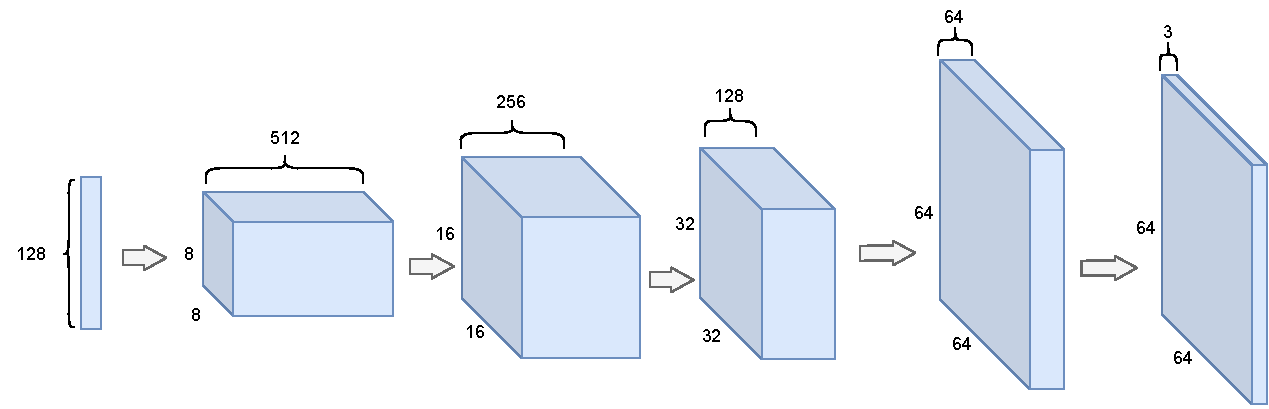
\includegraphics[width=\textwidth]{images/cnn3.pdf}
\end{figure}

\paragraph{Kostenfunktion} Als Kostenfunktion wird für die
Projekt-Implementierung entsprechend des \gls{acr-SNDCGAN} Papers die
ursprüngliche Standard-Kostenfunktion aus dem Paper von
\citeauthor{goodfellow2014generative} \cite{goodfellow2014generative} verwendet.
Diese ist gegeben als $V(D, G) = \mathbb{E}_{x \sim p_{\text{data}}(x)} [\log
D(x)] + \mathbb{E}_{z \sim p_{z}(z)} [\log (1-D(G(z)))]$. Dabei wird davon ausgegangen, dass der
Discriminator $D$ eine $1$ ausgibt, wenn er der Ansicht ist, dass das
eingegebene Bild sicher ein original Bild der Daten ist. Damit ist das Ziel des
Discriminators $V(D,G)$ zu maximieren, während der Generator die Funktion
minimieren möchte: $\min_{G} \max_{D} V(D,G)$. In der Praxis des Projektes wird,
ebenfalls dem \gls{acr-SNDCGAN} und \gls{acr-GAN} Papern folgend \cites{goodfellow2014generative}{miyato2018spectral}, statt der Minimierung
von $\log(1-D(G(z)))$, $\log D(G(z))$ maximiert, dies verringert das Problem von
verschwindenden Gradienten im frühen Training.

\paragraph{Training} Das Training der Projekt Implementierung folgt im
wesentlichen dem von \citeauthor{goodfellow2014generative}
\cite{goodfellow2014generative}. Der Generator und Discriminator werden jeweils
abwechselnd trainiert, wobei zuerst der Generator eine Batch von Beispiel-Daten
erzeugt, die anschließend vom Discriminator bewertet werden. Dies wird zuerst
für die Kosten des Generators verwendet und anschließend, zusammen mit einer
Bewertung von Originaldaten durch den Discriminator, für das Training des
Discriminators. Den Lernverfahren der einbezogenen Paper
\cite{radford2015unsupervised,miyato2018spectral,kurach2018gan} folgend,
verwendet die Implementierung des Projektes den Adam-Optimizer
\cite{kingma2014adam}.
 
 \subsection{Wasserstein-GAN} % Tim
 Das \gls{acr-WGAN} wurde 2017 in \citetitle{arjovsky2017wasserstein}
 \cite{arjovsky2017wasserstein} vorgestellt. Dabei verwendet dieses einen
 alternativen Weg um den Generator zu trainieren, welcher die Datenverteilung
 der gegebenen Trainingsdaten besser approximieren soll. Anstatt einen
 Discriminator zu verwenden, der Bilder in real oder nicht real kategorisiert,
 verwendet das \gls{acr-WGAN} einen einen \enquote{Critic}, welcher durch einen
 linearen Wert Bilder nach ihrem Realismus bewertet. 
 
 Für die Aufgabe Landschaftsbilder zu generieren wurde ebenfalls ein
 \gls{acr-WGAN} implementiert. Aufgrund fehlender Trainingsressourcen konnte
 diese Implementation jedoch nicht optimiert werden und liefert deutlich
 schlechtere Ergebnisse als die \gls{acr-SNDCGAN} Implementierung. Dennoch ist
 das \gls{acr-WGAN} eine interessante Möglichkeit ein Generator zu erschaffen.  
 
 \paragraph{Architektur} Die in diesem Projekt verwendete Architektur des
 \gls{acr-WGAN}s orientiert sich an der des \gls{acr-SNDCGAN}s, beschrieben in
 \cref{sub:sndcgan}. Allerdings wurden weniger Convolutions verwendet um
 Ressourcen zu sparen, da die Architektur noch nicht optimiert wurde. Der Critic
 verwendet ebenfalls Convolutions, und fügt diese am Ende zu einem linearen Output zusammen \cite{brownlee_how_2019-1}.
 Außerdem werden die Gewichte im Critic zwischen -0.01 und 0.01 beschränkt
 \cite{arjovsky2017wasserstein}. 
 
 \paragraph{Kostenfunktion} Das \gls{acr-WGAN} verwendet den Wasserstein-Loss,
 welcher versucht den Abstand zwischen realen und generierten Bildern zu
 maximieren. Dabei können die Kostenfunktionen nach \cite{brownlee_how_2019}
 folgendermaßen definiert werden:
 \begin{itemize}
 	\item Critic Loss = [Durchschnittlicher Critic Wert auf realen Bildern] –
 	[Durchschnittlicher Critic Wert auf generierten Bildern]
 	\item Generator Loss = -[Durchschnittlicher Critic Wert auf generierten
 	Bildern]
 \end{itemize}

\paragraph{Training} Einer der großen Vorteile des \gls{acr-WGAN}s ist, dass es
keinen Discriminator gibt, der dem Generator \enquote{davonläuft}. Ein besserer
Critic sorgt für bessere Ergebnisse \cite{arjovsky2017wasserstein}.
Deshalb wird beim Training der Critic mehr trainiert, als der Generator, in
diesem Fall fünf mal so oft. Zudem wird RMSProp statt Adam als Optimizer
verwendet \cite{arjovsky2017wasserstein}.
 
  \section{Implementierung} % Jonathan
  \label{sec:gen_impl}
 
 Der folgende Abschnitt thematisiert die Implementierung des zuvor beschriebenen
 SNDCGAN-Modells in Tensorflow bzw. Keras. Außerdem wird auch die Optimierung
 der Parameter der Netze behandelt.
 
 \subsection{Umsetzung in Tensorflow/Keras}\label{subsec:imp:sndc}
 
 Ein wichtiger Teil der Implementierung ist die Überführung der in
 Abschnitt~\ref{subsec:mod:sndc} vorgestellten Architektur des SNDCGANs in ein
 Tensorflow-Modell. Dafür wird das \glqq Sequential Model\grqq\ von
 Keras~\cite{keras:SequentialModel} verwendet. In dem Modell werden die
 benötigten Schichten des Generators und des Discriminators definiert. Beim
 Trainieren wird der Input sequenziell von einer Schicht zur nächsten
 durchgereicht und adaptiert, daher auch die Namensgebung.  
 
 Nachdem die Architektur des SNDCGANs zu Beginn des Projektes implementiert war,
 konnten erste Tests durchgeführt werden. Dabei war es ein großes Problem, dass
 der Fehler des Discriminators schnell auf null ging und damit der Generator
 keine Chance mehr hatte, irgendetwas zu lernen bzw. zu verbessern, da jeder
 Versuch als künstliches Bild enttarnt wurde und der Generator somit keine
 Erfolge mehr verbuchen konnte. Aus diesem Grund wurde die Architektur des
 Discriminators angepasst und Dropout eingeführt. Dadurch werden bei jedem
 Trainingsvorgang nur ein Teil der Neuronen trainiert und der Generator bekommt
 eine Chance, sich gegen den Discriminator durchzusetzen.
 
 Die komplette Implementierung der am Ende verwendeten Architektur beider
 Modelle ist im Anhang unter \autoref{lst:sndcGenerator} und
 \ref{lst:sndcDiscriminator} zu finden.
 
 Weiter wird für das Trainieren des SNDCGANs eine Trainingsschleife benötigt.
 Die in diesem Fall verwendete Schleife wurde zunächst aus \cite{raschka2019}
 übernommen und im Folgenden an die Bedürfnisse des Projektes angepasst. Um die
 Gradienten für ein anschließendes Gradientenabstiegsverfahren zu berechnen,
 werden GradientTapes von Tensorflow~\cite{tf:gradientape} eingesetzt. Diese
 speichern alle Operationen, die bei der Ausführung des zu trainierenden Netzes
 durchgeführt werden und können daraus dann die Gradienten
 berechnen~\cite{tf:autodiff}.
 
 Um die neuronalen Netze zu optimieren, wird der Adam Algorithmus eingesetzt.
 Dieser führt einen Gradientenabstieg durch und wird bereits von Tensorflow zur
 Verfügung gestellt~\cite{tf:adam}. Als Besonderheit bringt Adam u. a. eine über
 die Zeit abnehmende Lernrate mit~\cite{kingma2014}.
 
 Ein weiterer wichtiger Teil der Implementierung ist die Möglichkeit, das
 Training zu pausieren und später wieder an gleicher Stelle aufzunehmen. Dies
 war vor allem wichtig, da die Rechenkapazitäten für dieses Projekt sehr
 begrenzt waren, somit das Trainieren viel Zeit in Anspruch genommen hat und das
 Training dabei nicht an einem Stück durchgeführt werden konnte. Deshalb wurde
 implementiert, dass in regelmäßigen Abständen Checkpoints des Lernfortschritts
 gespeichert werden. Diese Umfassen neben den Modellen des Generators und
 Discriminators auch deren Optimizer. Dies ist wichtig, da wie zuvor erwähnt
 wurde, die Lernrate der Adam Optimizer über die Zeit abnimmt. Somit ist nur
 eine Fortsetzung des Trainings beim gleichen Stand möglich, wenn auch die
 bisher verwendeten Optimizer geladen werden. 
 
 Zunächst war geplant, dass diese Checkpoints dauerhaft gespeichert werden,
 damit die trainierten Netzwerke später ausgewertet und verwendet werden können.
 Bei Testläufen hat sich allerdings herausgestellt, dass jeder Checkpoint fast
 600 MB umfasst und dies sich dann über die ganzen Epochen zu einem großen
 Speicherverbrauch aufsummiert. Deshalb wurde zusätzlich eingeführt, dass die
 trainierten Modelle einzeln gespeichert werden und von den Checkpoints nur noch
 die letzten zwei erhalten bleiben. Dadurch konnte der Speicherplatz pro
 gespeicherter Epoche um zweidrittel reduziert werden.
 
 \subsection{Anpassung von Parametern} % Jonathan
 
 Eine große Herausforderung in diesem Projekt war die richtige Wahl der
 Parameter für das Training. Diese müssen so gewählt werden, dass das neuronale Netz möglichst gut
 initialisiert wird, um dann gute Ergebnisse zu produzieren. Dabei war das
 Hauptproblem die fehlende Rechenkapazität, um verschiedene Konfigurationen
 ausführlich auszutesten, anschließend mit einer wissenschaftlichen
 Herangehensweise zu vergleichen und daraus die besten Parameter abzuleiten. Aus
 diesem Grund mussten die Entscheidungen auf Basis weniger Versuche getroffen
 werden. Daher ist es mit Sicherheit möglich, anhand einer ausführlicheren
 Analyse besser passende Parameter zu finden.
 
 Im Folgenden werden die vier Variablen \emph{Droprate}, \emph{initiale
 Lernrate}, \emph{Bildermenge} und \emph{Auflösung der Bilder} genauer
 thematisiert.
 
 Wie im vorherigen Abschnitt~\ref{subsec:imp:sndc} bereits erwähnt wurde, war es
 zu Beginn des Projektes ein großes Problem, dass der Fehler des Discriminators
 nach kurzer Zeit auf null ging und damit einen Lernfortschritt des Generators
 unmöglich machte. Neben der Einführung des Dropouts, war auch die Anpassung der
 initialen Lernrate auf der Seite des Discriminators wie auch auf der des
 Generators eine wichtige Stellschraube. Während es bei der Droprate auf Basis
 eines Blogbeitrags~\cite{brownlee2019} relativ schnell möglich war, einen Wert
 von 50 \% festzulegen, mussten bei der Lernrate einige Testläufe absolviert
 werden. 
 
 Die zu Beginn gewählten Lernraten bewegten sich in der Größenordnung von E-3
 und mit ihnen trat das Verschwinden des Discriminator-Fehlers auf. Eine
 Vergrößerung der Lernrate wirkte sich deutlich negativ auf das Lernverhalten
 aus, da der Fehler des Discriminators noch schnell zu null ging. Als dritten
 Ansatz wurden unterschiedliche Lernraten für Generator und Discriminator
 getestet. Dabei wurde die des Generators im Bereich von E-3 deutlich größer
 gewählt als die des Discriminators mit E-4. Das Ziel war, den Generator
 schneller lernen zu lassen, als den Discriminator. Allerdings waren die
 Ergebnisse damit auch noch nicht zufriedenstellend. Erst ein Reduzieren beider
 Lernraten in den Bereich von E-4 hat für sichtbare Veränderungen bei den
 produzierten Beispielbildern gesorgt.
 
 Um den Trainingsprozess bei diesen Versuchen zu beschleunigen, wurde immer nur
 mit relativ wenig Bildern gelernt. Erst nachdem die ersten Erfolge durch eine
 bessere Wahl der initialen Lernrate sichtbar wurden, erhöhte sich die
 Bildermenge auf zunächst ca. 1500 Stück und später dann auf etwas mehr als
 7000, was auch eine weitere Verbesserung der Ergebnisse mit sich brachte.
 Allerdings beschränkten sich die Verbesserung auf sichtbare Änderungen in den
 abgebildeten Formen, die zunehmend komplexer wurden. Die erstellten Bilder
 hatten jedoch noch wenig Ähnlichkeit zu (schlecht aufgelösten)
 Landschaftsbildern.
 
 Die letzte Änderung, die anschließend zu zufriedenstellenden Ergebnissen
 geführt hat, war eine Vergrößerung der Auflösung. Das bis dahin mit einer
 Bilderauflösung von 128x72 Pixeln trainierte SNDCGAN wurde auf 256x144 Pixel
 vergrößert. Dies bedeutete zwar einen deutlich Anstieg der Rechenzeit,
 allerdings war damit in den Beispielbildern mehr Inhalt zu erkennen, den das
 GAN lernen konnte.
 
 \section{Evaluierung}\label{evalGen} Nachdem das Training des implementierten
  GANs erfolgreich abgeschlossen wurde, erfolgt die Evaluation der Ergebnisse.
  Dafür wurden zwei verschieden Methoden genutzt. Die Erste betrachtet den
  durchschnittlichen Loss des Generators und Discriminators, zu sehen in
  Abbildung \ref{fig:plot_losses_gen}.  Hier ist zu erkennen, dass zu Beginn
  Spitzen von großen Losses auftreten, diese sich aber im Verlauf zu späteren
  Epochen auspendeln und zu einem Minimum tendieren. Daraus kann gefolgert
  werden, dass die Netze ihre Aufgabe erfüllen, nämlich die Losse beider Netze
  zu minimieren. In den letzten hundert Epochen ist eine steigende Tendenz zu
  beobachten, die auf ein Overfitting zurückgeführt werden kann.
 
 \begin{figure}[t]
 	\centering
 	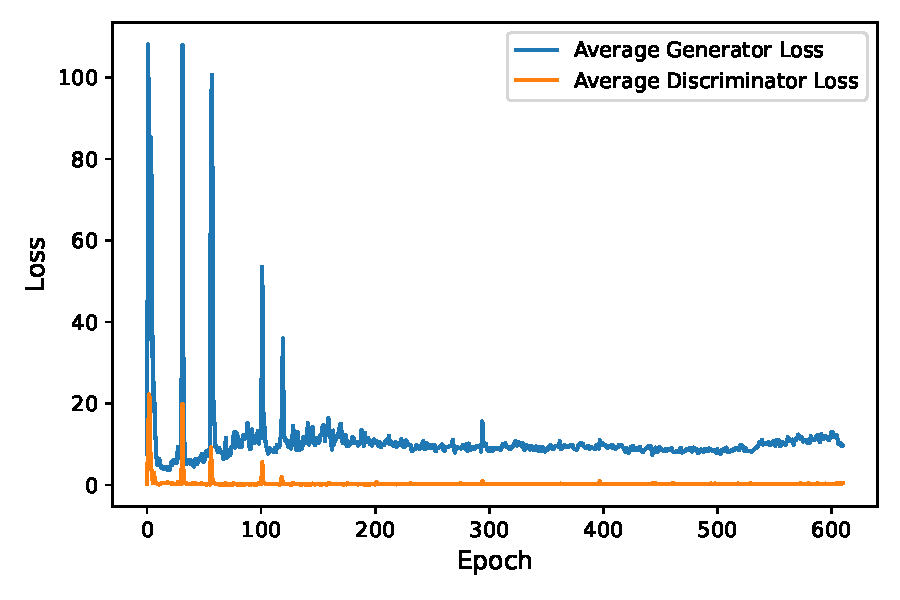
\includegraphics[width=0.7\linewidth]{images/plot_line_plot_losses_gen}
 	\caption[Losses des generirenden GANs]{Der Loss über alle Epochen des GANs , welches für das generieren von Landschaftsbilder genutzt wurde.}
 	\label{fig:plot_losses_gen}
 \end{figure}
 
 Die zweite Methode ist das Berechnen der \acrfull{acr-FID}. Diese bestimmt die
 Ähnlichkeit der echten und der generierten Bilder \cite{heusel_gans_2017}. Dies
 wird über die Fr\'echet Distanz gemacht, welche die Gaußglocken der
 Verteilungen beider Domänen vergleicht. Die Gaußglocke wird über den Mittelwert
 $m$ und die Kovarianz $C$ festgelegt. 
 
 \[d^2((m,C),(m_w,C_w)) =  \|m-m_w\|^2_2 + trace(C+ C_w - 2(CC_w)^{\frac{1}{2}})
 \]
 
 Die in dieser Arbeit umgesetzte Implementierung von \gls{acr-FID} geht über
 alle gespeicherten Modelle des Generators (hier jede fünfte Epoche). Anhand dieser
 werden  
 mittels über alle Epochen gleichbleibenden Zufallsvektoren Bilder generiert.
 Diese Bilder werden nun mit einer zufälligen aber festen Auswahl an echten
 Bilder verglichen, in dem alle Bilder durch den besten Discriminator bewertet
 werden. Beim Discriminator müssen die letzten beiden Schichten entfernt werden
 und durch eine Pooling-Schicht mit anschließendem Abflachen ersetzt werden,
 damit die Berechnung der Mittelwerte und Kovarianzen durchgeführt werden kann. 
 
 Die Auswertung des genutzten Modells unter Verwendung des Discriminators mit
 geringsten Loss ist in Abbildung \ref{fig:plot_fids_gen} sichtbar. Über die
 Approximation ist klar zu erkennen, dass der Wert im Laufe der Zeit fallend
 ist, was eine Annäherung der generierten Bilder zu den echten Bilder
 widerspiegelt. Genau diese Eigenschaft ist bei der Generierung mittels GANs
 gewünscht.
 
 \begin{figure}
 	\centering
 	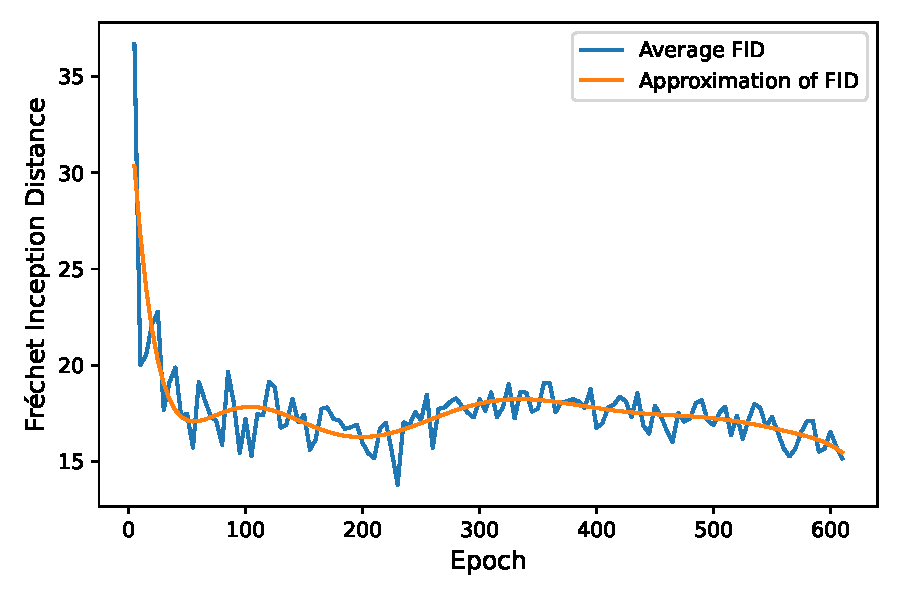
\includegraphics[width=0.7\linewidth]{images/plot_line_plot_fids_gen}
 	\caption[FID des generierdene GANs]{FID über alle Epochen mit dem Discriminator aus Epoche 535}
 	\label{fig:plot_fids_gen}
 \end{figure}
 
 Das Fazit aus den beiden Evaluierungsmethoden ist, dass das in dieser Arbeit
 implementierte und trainierte GAN die Aufgabe des Generierens von
 Landschaftsbilder gut umgesetzt hat. Die Losses des gesamten Netzes pendeln
 sich auf feste Werte ein, bei denen es sich um das Minimum handelt. Sowie die
 Ergebnisse der \gls{acr-FID} zeigen, dass die generierten Bilder relativ ähnlich
 zu echten Bilder sind, wodurch die generierten Bilder für den Menschen wie
 echte Landschaftsbilder wirken.
 %TODO: Bilder vergleich zeigen?
 
 
\chapter{Manipulieren von Bildern}\label{chp:bildmanipulation} %10 Seiten
\glsresetall

Neben dem Erzeugen von Landschaftsbildern (\cref{chp:bildgenerierung}), ist der
zweite Teil dieses Projektes das Manipulieren der Bilder. Das Ziel ist es,
Landschaftsbilder zu verschiedenen Tageszeiten zu erhalten. Dafür soll der
Inhalt der Eingabe beibehalten werden,  der Stil des Bildes sich aber der
Tageszeit anpassen. Zum Beispiel soll aus einem Bild am Tag ein Bild bei Nacht
werden.
 
 \section{Modelle} % Dani
 Für das Manipulieren von Bildern gibt es verschieden Ansätze (vgl. \cref{GANsBildmanipulation}). Eingegrenzt
 wurden diese durch den genutzten Datensatz. Da die Bilder hier nicht in Paaren vorliegen, es
 also zu einem Eingabebild keine entsprechendes Bild in der Zieldomain gibt,
 muss ein unsupervised Verfahren verwendet werden.
 Im Rahmen dieser Arbeit werden zwei Ansätze genauer betrachtet. Der erste
 Ansatz ist der des CycleGANs \cite{zhu2017unpaired}, welches mittels des Cycle
 Consistency Losses versucht Bilder zwischen zwei Domänen zu transferieren. Der
 zweite Ansatz heißt  \gls{acr-funit} \cite{liu2019few}. Dieser orientiert sich am
 Vorgehen des menschlichen Gehirns und versucht mit wenigen Bildern aus
 ähnlichen Domänen die Übersetzung zu lernen.
 
 \subsection{CycleGAN}% Dani
 \label{sub:cyclegan}
 Durch das Fehlen von gepaarten Bildern, fehlt eine Möglichkeit zu überprüfen, ob der Generator den Inhalt des Bildes beibehält. \citeauthor{zhu2017unpaired} \cite{zhu2017unpaired} lösen dieses Problem durch Einfügen einer weiteren Bedingung: Bilder sollen, wenn sie übersetzt wurden und anschließen wieder zurück umgewandelt werden, gleich sein bzw. sehr ähnlich. Dies wird mittels des Cycle Consistency Losses umgesetzt. 
 Dazu benötigt man zwei GANs: Eines, welches aus der Eingabedomäne in die Zieldomäne übersetzt, $G: X \rightarrow Y$, und ein Anderes, welches das Gegenteil bewirkt,   $F: Y \rightarrow X$.
 Der Cycle Consistency Loss beschreibt die Größe des Unterschiedes zwischen dem
 ursprünglichen Bild und dem wiederhergestellten Bild, welches durch das
 sequentielle Anwenden der beiden GANs entsteht. 
 Das Ziel ist es $F(G(X))\approx X$ sowie $G(F(Y))\approx Y$ durchzusetzen. Dies
 ist in Abbildung \ref{fig:cylce_loss} dargestellt. Der Verlust wird dabei jeweils
 zwischen
 $x$, $\hat{x}$ und $y$,$\hat{y}$ berechnet.
 Die jeweiligen GANs lernen dazu noch über den Adversarial Loss, also dem Feedback des jeweiligen Discriminators des GANs. 
 Dadurch ergibt sich der Verlust des CycleGANs als:
 \[ \mathcal{L}(G,F,D_X,D_Y) = 	\mathcal{L}_{GAN}(G,D_Y,X,Y) + 	\mathcal{L}_{GAN}(F, D_X,Y,X) +\lambda 	\mathcal{L}_{cyc}(G,F)   \]
 Dabei sind $D_X$ und $D_Y$ die Discriminators für die jeweilige Domäne und
 $\lambda$ legt die Wichtigkeit des Cycle Consistency Losses fest. 
 Das Zeil des Lernens ist es 
 \[G^*,F^* = arg \min_{G,F} \max_{D_X,D_Y} \mathcal{L}(G,F,D_X,D_Y) \] zu lösen.
 
 \begin{figure}
 
 	\tikzstyle{block} = [draw=black, thick, text width=1cm, minimum height=1cm, align=center]  
 	\tikzstyle{line} = [draw=black, thick, text width=1cm, minimum height=3cm, align=center]  
 	\begin{tikzpicture}
 		
 		\node[block] (a) {$x$};
 		\node[block, right=of a] (b) {$\hat{Y}$};
 		\node[block, right=of b] (c) {$\hat{x}$};
 		\node (Dy) [above of=b] {$D_Y$};
 		
 		\node[block, right=of c] (d) {$y$};
 		\node[block, right=of d] (e) {$\hat{X}$};
 		\node[block, right=of e] (f) {$\hat{y}$};
 		\node (Dx) [above of=e] {$D_X$};
 		
 		\path [thick,->,>=stealth]
 		(a) edge [bend left] node [above] {$G$} (b)
 		(b) edge [bend right] node [above] {$F$} (c)
 		(d) edge [bend right] node [above] {$F$} (e)
 		(e) edge [bend left] node [above] {$G$} (f);
 		
 		\draw[dashed,->] (b) to node [] {} (Dy);
 		\draw[dashed,->] (e) to node [] {} (Dx);
 		
 		\draw ([yshift=0.7cm]$(c.north east)!.5!(d.north west)$) --([yshift=-0.7cm]$(c.south east)!.5!(d.south west)$);
 	\end{tikzpicture}
 	\caption[cycle consistency loss]{Cycle Consistency Loss in beide Richtungen}
 	\label{fig:cylce_loss}
 \end{figure}
 
 Die Architektur der genutzten Netze stammt von \citeauthor{johnson_perceptual_2016} \cite{johnson_perceptual_2016}. Für den Generator gibt es zwei Varianten, die eine für Eingabegröße $128 \times 128$ mit 6 Residual Blöcken und die andere für Eingabegröße $256 \times 256$ mit 9 Residual Blöcken (ResBlock). Diese Blöcke führen zwei Convolutions mit gleicher Anzahl an Filtern aus. Als Normalisierung wird Instance Normalisierung genutzt, diese ist eine Erweiterung der Batch Normalisierung \cite{ulyanov_instance_2016}. In \cref{tab:cycleGAN} ist der Aufbau der Generators und der Discriminatoren für die Variante mit Eingabegröße $256 \times 256$ zu sehen.
 
 \begin{table}[]
 	\caption{CycleGAN Architektur}
 	\label{tab:cycleGAN}
 	\begin{center}
 		\begin{minipage}{.5\linewidth}
 			\caption{CycleGAN Discriminator}
 			\centering
 			\begin{tabular}{lcl}
 				\toprule
 				Schicht & Kernel & Filter\\
 				\toprule
 				Conv, lReLU & $[4,4,2]$ & $64$\\
 				\midrule
 				Conv, IN, lReLU & $[4,4,2]$ & $128$\\
 				\midrule
 				Conv, IN, lReLU & $[4,4,2]$ & $256$\\
 				\midrule
 				Conv, IN, lReLU & $[4,4,2]$ & $512$\\
 				\midrule
 				Conv & &$1$\\
 				\bottomrule
 			\end{tabular}
 		\end{minipage}%
 		\begin{minipage}{.5\linewidth}
 			\centering
 			\caption{CycleGAN Generator}
 			\begin{tabular}{lcl}
 				\toprule
 				Schicht & Kernel & Filter\\
 				\toprule
 				Conv, IN, ReLU & $[7,7,1]$ & $64$\\
 				\midrule
 				Conv, IN, ReLU & $[3,3,2]$ & $128$\\
 				\midrule
 				Conv, IN, ReLU & $[3,3,2]$ & $256$\\
 				\midrule
 				ResBlock & $[3,3,1]$& $256$ \\
 				\midrule
 				ResBlock & $[3,3,1]$& $256$ \\
 				\midrule
 				ResBlock & $[3,3,1]$& $256$ \\
 				\midrule
 				ResBlock & $[3,3,1]$& $256$ \\
 				\midrule
 				ResBlock & $[3,3,1]$& $256$ \\
 				\midrule
 				ResBlock & $[3,3,1]$& $256$ \\
 				\midrule
 				ResBlock & $[3,3,1]$& $256$ \\
 				\midrule
 				ResBlock & $[3,3,1]$& $256$ \\
 				\midrule
 				ResBlock & $[3,3,1]$& $256$ \\
 				\midrule
 				DeConv, IN, ReLU & $[3,3,2]$ & $128$\\
 				\midrule
 				DeConv, IN, ReLU & $[3,3,2]$ & $64$\\
 				\midrule
 				Conv, IN, ReLU & $[7,7,1]$ & $3$\\
 				\bottomrule
 			\end{tabular}
 		\end{minipage} 
 	\end{center}
 	\begin{center}
 		\bigskip
 		\emph{Quelle:} Von \cite{zhu2017unpaired} übernommen.\\
 		\emph{Legende:} Der Kernel ist beschrieben im Format $[\text{x\_Größe},
 		\text{y\_Größe}, \text{Schrittweite}]$;IN steht für InstanceNorm; LeakyReLu hat eine Neigung von $0,2$.
 	\end{center}
 \end{table}
 
 
 Durch Evaluierungen und Vergleiche konnten \citeauthor{zhu2017unpaired} beobachten, dass die wiederhergestellten Bilder und die echten Bilder ein gute Ähnlichkeit aufwiesen. Vor allem bei Manipulationen bei denen Farben und Texturen geändert werden, wie es für die Veränderung von Landschaftsbildern der Fall wäre. 
 
 \subsection{FUNIT}% Dani
 \label{sub:funit}
 Der Ansatz von \citeauthor{liu2019few} \cite{liu2019few}  geht das Problem an, dass es oft nicht genug Bilder in den Eingabe- und Zielklassen gibt. Dazu wurde eine Methode, die nur wenige Eingabedaten benötigt (few-shot) entwickelt. Hierbei wird das Modell mit Bildern aus verschieden Eingabeklassen trainiert und erst beim Testen werden die Bilder der Zielklasse genutzt.
 Dazu wurde eine neues Netzwerkdesign mit dem kompetitiven Training von GANs vereinigt. Der Name diese Modells ist  \acrfull{acr-funit}. Dieses Netzwerk besteht aus insgesamt vier Teilnetzen, drei im Generator und eins im Discriminator. Der Generator $G$ bekommt als Eingabe ein Bild $x$ aus der Klasse $C_x$ und eine Reihe von Bildern $y_1,\dots,y_n$ aus einer anderen Eingabeklasse $C_y$. Die Ausgabe $\hat{x}$ sollte dann der Inhalt von Bild $x$ in dem Stil der Klasse $K_y$ sein. 
 Die drei Netze, die zusammen den Generator ergeben, sind der Inhalt-Encoder $E_x$, der Klassen-Encoder $E_y$ und der Decoder $F_x$.
 Der Inhalt des Eingabebilds $x$ wird durch den Inhalt-Encoder in eine räumliche Feature-Map umgewandelt. Die andern Eingabebilder $y_1,\dots,y_n$ werden in den Klassen-Encoder gegeben, der jedes Bild auf einen Latenten Mittel Vektor (\emph{intermediate latent vector}) abbildet und anschließend den Mittelwert über alle Vektoren berechnet, zu sehen in Abbildung \ref{fig:funitmodelsimple}. 
 Mit den Ausgaben aus den beiden Encodern konstruiert der Decoder das Ausgabebild des Generators. 
 \[\hat{x} = G(x, y_1,\dots,y_n)= F_x(E_x(x), E_y(y_1,\dots,y_n))\]
 
 Der Discriminator $D$ hat für jede Klasse die Aufgabe zu entscheiden, ob ein Bild echt ist oder durch den Generator erzeugt wurde. Es wird nur bestraft, wenn bei einem echten Bild nicht die richtige Klasse erkannt wird und wenn ein generiertes Bild der Zielklasse zugeordnet wird. Der Generator bekommt nur dann eine Bestrafung, wenn das generierte Bild nicht der gewünschten Klasse zugeordnet wurde.
 
 Beim Lernen wird das lösen folgender Gleichung versucht:
 
 \[\min_{D} \max_{G} \mathcal{L}_{GAN}(D,G) + \lambda_R \mathcal{L}_R(G) + \lambda_F \mathcal{L}_{F}(G) \]
 
 wobei $ \mathcal{L}_{GAN}(D,G)$ für den Loss des gesamten GANs, $ \mathcal{L}_R(G)$ für den der Bildinhaltswiederherstellung und $\mathcal{L}_{F}(G) $ den der Feature-Abstimmung  steht. 
 
 Bei Vergleichen mit anderen gängigen Ansätzen, schnitt  \gls{acr-funit}  besser ab und benötigt dabei einen kleineren Datensatz \cite{liu2019few}. Diese beiden Vorteile bieten sich für die Manipulation, die in dieser Arbeit durchgeführt werden soll, an.
 
 \begin{figure}[h]
 	\centering
 	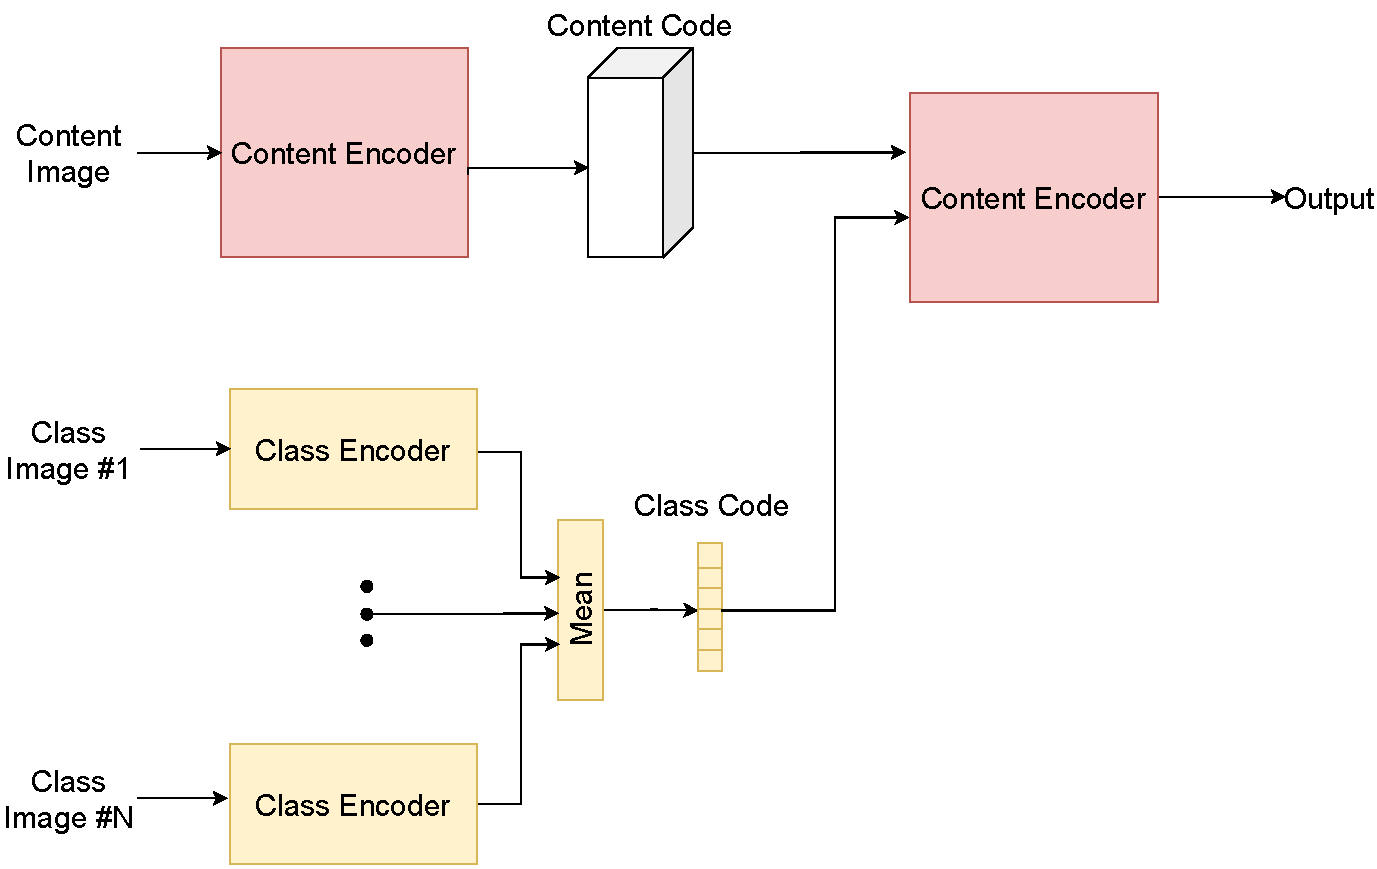
\includegraphics[width=0.8\linewidth]{images/Funit_Model_simple}
 	\caption[Modell FUNIT]{Modell des Generators von FUNIT}
 	\label{fig:funitmodelsimple}
 \end{figure}
 

 
 \section{Implementierung} % Tim nach Implementierung Generieren
  Für die Implementierung der Bildmanipulation benutzt das Projekt, aufgrund des Datensatzes und der beschränken Rechenleistung, das CycleGAN. Dieses wurde mit Tensorflow und Keras umgesetzt. Da dieses GAN deutlich größer als das \gls{acr-SNDCGAN} (siehe \cref{subsec:mod:sndc}) ist, konnte es, aufgrund der beschränkten Computerressourcen, nur einmal trainiert werden. Alle Trainingsparameter wurden vorher festgelegt, wobei die Erfahrungen aus \cref{sec:gen_impl} genutzt wurden.
 
 \subsection{Umsetzung in Tensorflow/Keras}
 Wie auch für das \gls{acr-SNDCGAN} wurde ein \enquote{Sequential model} von Keras~\cite{keras:SequentialModel} verwendet um die einzelnen Schichten abzubilden. Da nicht alle benötigten Netzschichten in Keras  vorimplementiert sind, mussten zudem für die \texttt{ResBlock} und \texttt{ReflectionPadding2D} Schichten \cite[vgl.][]{zhu2017unpaired}, sowie für \texttt{Tanh},  eigene Klassen geschrieben werden, welche von einer abstrakten Keras Schicht erben. 
 
 Das Training des CycleGAN wurde ähnlich wie das des \gls{acr-SNDCGAN} in \cref{sec:gen_impl} implementiert. Ebenfalls wurde es durch Checkpoints ermöglicht das Netz jederzeit anzuhalten und später weiter zu trainieren. Adam \cite{tf:adam} wurde als Optimizer und GradientTapes \cite{tf:gradientape} zur Berechnung der Gradienten verwendet.
 
Die Optimizer sind identisch parametrisiert und wurden wie in der Implementierung von \cite{brownlee_how_2019-1} auf eine Lernrate von 2e-4 und ein \texttt{beta1} von 0.5 gesetzt. 

Da das CycleGAN aus vier mehrschichtigen Netzen besteht, welche zusammen trainiert werden, ist das Training sehr speicherintensiv. Nur dadurch, dass einzelne Trainingsschritte in eine Funktion mit dem \texttt{tf.function} Decorator \cite{noauthor_tffunction_nodate} ausgelagert sind, kann die stärkste dem Projekt zur Verfügung stehende Grafikkarte genug Speicher bieten, um das Training – mit einer geringen Batchgröße – durchzuführen. 


 \section{Evaluierung} % TODO Tim und Joshua
 
 Das CycleGAN wurde 625 Epochen trainiert, dabei sind die Ergebnisse allerdings nicht 
 zufriedenstellend. In \cref{fig:sub-dogtocat} und \ref{fig:sub-cattodog} kann man jeweils ein 
 Eingabebild und das Ausgabebild für die Transformationen Hund zu Katze bzw. Katze zu Hund 
 sehen. Es gibt mehrere wahrscheinliche Gründe für die relativ schlechten Ergebnisse. Zum einen 
 zeigen die beiden Trainingsbilderdatensätze Hunde und Katzen von verschiedenen Perspektiven. 
 Ein weiteres Problem des Bilderdatensatzes ist, dass die Bilder unterschiedliche Hintergründe 
 haben, was kombiniert mit unterschiedlich großen Tieren und Perspektiven das Netz 
 \enquote{verwirren} kann. Für diese Probleme wäre \gls{acr-funit} besser geeignet als das 
 CycleGAN 
 \cite{liu2019few}. Hier wäre es interessant das CycleGAN, wie ursprünglich geplant, mit
 Landschaftsbildern zu trainieren, da diese keine Perspektiven und Hintergrundprobleme aufweisen. 
 Leider war dies aufgrund fehlender Bilderkategorien nicht möglich. Zudem konnte durch die 
 limitierte Rechenleistung das GAN nur mit einer Batchgröße von 4 trainiert werden. Eine höhere 
 Batchgröße hilft beim Generalisieren der Trainingsbilder. 
 
 Dennoch kann man mithilfe der Loss-Werte in \cref{fig:cycleganloss} erkennen, dass das CycleGAN 
 Fortschritte macht. Interessant ist hier, dass nach etwa 450 Epochen der Loss wieder steigt. Dies 
 liegt vermutlich an dem Auftreten von Overfitting. 


 Als objektive Metrik für die Evaluierung der
 Bildmanipulation wird eine \emph{\gls{acr-PD}} \cite{pang2021image} verwendet, die aus dem
 \emph{Perceptual Feature Reconstruction Loss} von
 \citeauthor{johnson_perceptual_2016} \cite{johnson_perceptual_2016} abgeleitet ist. Dazu wird, ähnlich der
 \gls{acr-FID} (vgl. \cref{evalGen}), die Aktivierung einer versteckten Schicht eines
 Bildklassifizierungsnetzes verglichen. In diesem Fall wird die 16-Schichten
 Variante des \emph{VGG} Netzes \cite{simonyan2014very} verwendet, welches auf
 dem ImageNet \cite{russakovsky2015imagenet} Datensatz trainiert wurde. Von diesem
 wird konkret die Aktivierung der drittletzten Convolution Schicht betrachtet.
 Die \gls{acr-PD} für zwei Bilder $x$ und $y$ berechnet sich dann als:
 \begin{displaymath}
	pd(x,y) = \frac{1}{HWC} ||\phi(x) - \phi(y)||_2^{2}
 \end{displaymath}
 Dabei ist $\phi(x)$ die Aktivierung der drittletzten
 Schicht des VGG Netzes bei Eingabe $x$ und $H \times W \times C$ das Format
 der Aktivierung. Die Aktivierung einer tieferen
 Convolution Schicht eines Klassifikationsnetzes, wie sie hier verwendet wird,
 ermöglicht es Bilder auf die Unterschiede im Inhalt zu vergleichen, wobei
 Unterschiede im Stil weitestgehend ignoriert werden
 \cite{johnson_perceptual_2016,pang2021image}. Daher ist diese Distanz als
 Metrik geeignet, um die erfolgreiche Übertragung des Bildinhaltes durch ein
 Image-to-Image Translation GAN zu bewerten.
 
 Die Ergebnisse der Metrik für das trainierte CycleGAN, sind in den Abbildungen \ref{fig:sub-dogtocatpd} und \ref{fig:sub-cattodogpd} zu finden. 
 Man kann über den Verlauf eine kleine Minderung der Distanz erkennen. Der Anstieg nach ungefähr 
 450 Epochen stimmt mit dem des Losses überein. Die niedrigen Startwerte sind jedoch unerwartet und 
 konnten nicht geklärt werden. 
 
 
 
 
 \begin{figure}[ht]
 	\centering
 	\begin{subfigure}{\textwidth}
 		\centering
 		% include first image
 		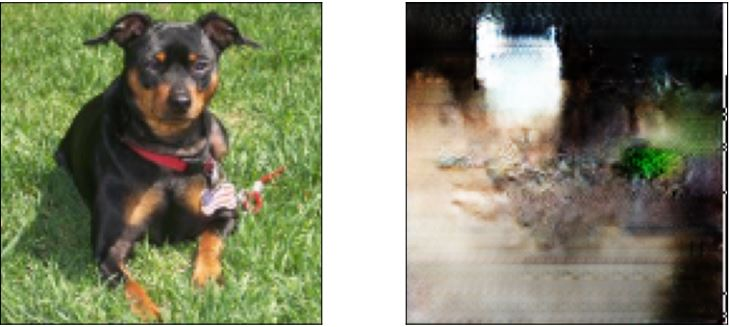
\includegraphics[width=.8\linewidth]{images/dogToCat}  
 		\caption{Transformation Hund zu Katze}
 		\label{fig:sub-dogtocat}
 	\end{subfigure}
 	\newline
 	\begin{subfigure}{\textwidth}
 		\centering
 		% include second image
 		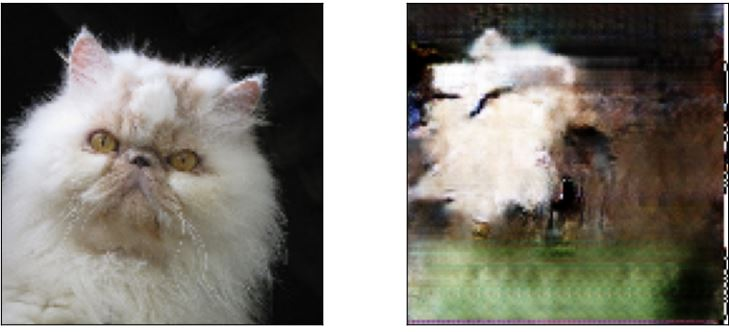
\includegraphics[width=.8\linewidth]{images/catToDog}  
 		\caption{Transformation Hund zu Katze}
 		\label{fig:sub-cattodog}
 	\end{subfigure}
 	\caption{Beispiel-Ergebnisse des CycleGANs}
 \end{figure}
 
 \begin{figure}
 	\centering
 	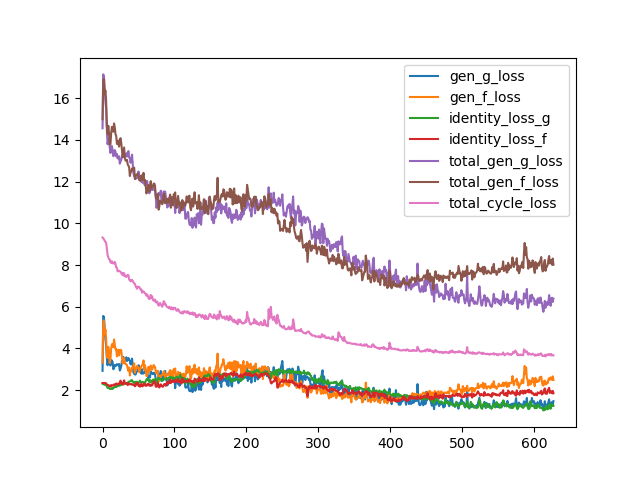
\includegraphics[width=0.7\linewidth]{images/plot_line_plot_loss}
 	\caption{\centering Loss über alle Epochen des CycleGAN Trainings}
 	\label{fig:cycleganloss}
 \end{figure}
 
  \begin{figure}[ht]
 	\centering
 	\begin{subfigure}{\textwidth}
 		\centering
 		% include first image
 		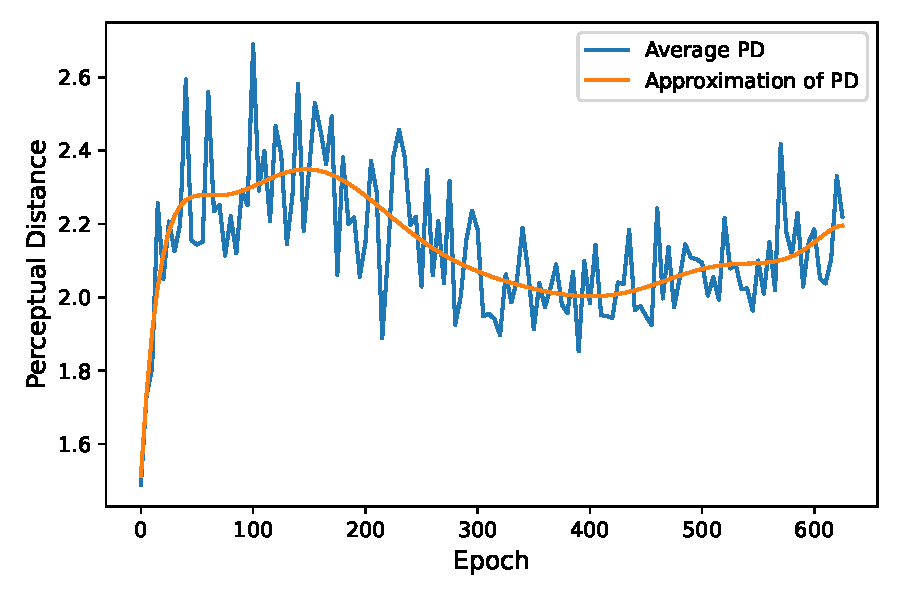
\includegraphics[width=.8\linewidth]{images/plot_line_plot_fidsdogcat}  
 		\caption{PD zwischen Hundebildern und den daraus generierten Katzenbildern}
 		\label{fig:sub-dogtocatpd}
 	\end{subfigure}
 	\newline
 	\begin{subfigure}{\textwidth}
 		\centering
 		% include second image
 		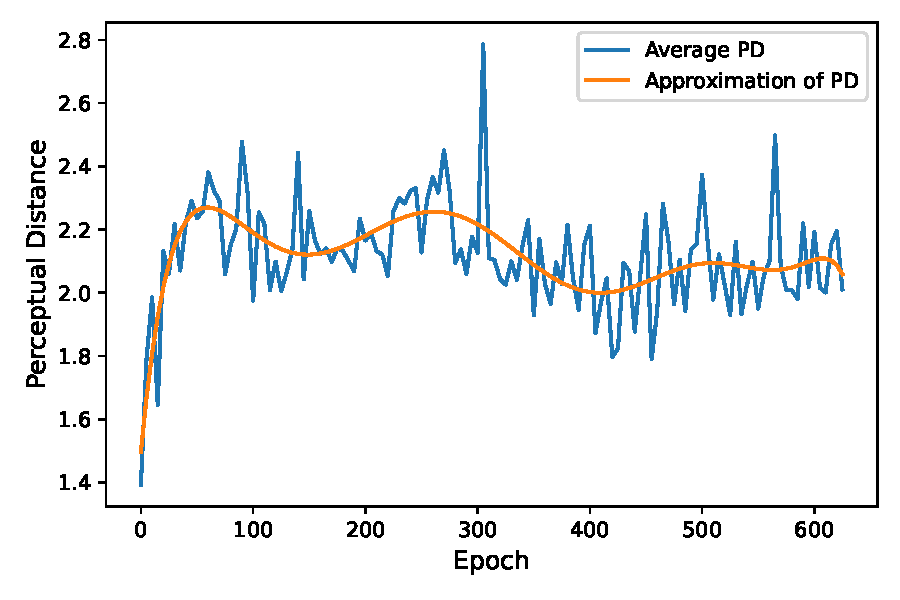
\includegraphics[width=.8\linewidth]{images/plot_line_plot_fidscatdog}  
 		\caption{PD zwischen Katzenbildern und den daraus generierten Hundebildern}
 		\label{fig:sub-cattodogpd}
 	\end{subfigure}
 	\caption{Auswertung der Perceptual Distance (PD) für das trainierte CycleGAN}
 	\label{fig:fig}
 \end{figure}
\chapter{Fazit}\label{chp:fazit} % Dani
\glsresetall

Die Motivation dieser Projektarbeit war es dynamische Wallpaper, die sich je nach 
Tageszeit verändern, zu generieren. Dafür sollte jeweils ein Generative Adversarial Network (GAN) für das 
Erzeugen von Landschaftsbildern und eines für das Manipulieren dieser Bilder 
implementiert werden. 

Leider gab es einige größere Hindernisse, wodurch gerade beim 
Manipulieren die Ergebnisse nicht praktisch einsetzbar sind. Zum einen ist es eine große 
Herausforderung einen geeigneten Bilderdatensatz zu finden bzw. zu erzeugen. Zum 
anderen benötigt das Trainieren bei den hier verwendeten Netzen sehr viel Rechenleistung 
und moderne Hardware, um überhaupt zu laufen. Diese Hindernisse sind besonders beim 
Bildmanipulieren relevant, da dort die Netze größer sind und zwei Bilderdatensätze 
benötigt werden. Somit wurde aufgrund fehlender Bilder das Bild-manipulierende 
\gls{acr-GAN} mit Hunde- und Katzenbildern trainiert. Zudem war es mit der zur Verfügung 
stehenden Hardware nicht möglich komplexere Netze wie das in \cref{sub:funit} 
beschriebene \gls{acr-funit} Netzwerk zu verwenden. Da Trainingszeiten bei mehreren 
hundert Stunden liegen konnten, war es außerdem schwierig verschiedene Ansätze zu 
verfolgen und die Trainingsparameter zu optimieren. 

Das Erstellen eines großen Bilderdatensatzes für das Bildgenerieren war ebenfalls sehr 
aufwendig, da alle Landschaftsbilder-Datensätze viele schlechte Bilder enthielten und 
deshalb manuell gefiltert werden mussten. 

Für das Generieren von Landschaftsbildern wurde schlussendlich ein \gls{acr-SNDCGAN} 
verwendet. Dieses wurde mit über 7000 Hand sortierten Landschaftsbildern trainiert. 
Dabei sind die generierten Landschaftsbilder auch als solche zu erkennen. Auffällig war, 
dass bei einer Bildauflösung von 128x72 Pixeln die Ergebnisse deutlich schlechter als 
mit der Auflösung 256x144 sind. Hier wäre es interessant das Training mit einer noch 
höheren Auflösung (auf besserer Hardware) abzuhalten und die Ergebnisse zu vergleichen. 
Zusätzlich zum  \gls{acr-SNDCGAN}  wurde auch ein \gls{acr-WGAN} implementiert. Da 
das \gls{acr-SNDCGAN} in ersten Versuchen jedoch besser abgeschnitten hat und die 
Hardwareressourcen begrenzt waren, wurde das \gls{acr-WGAN} nicht optimiert. Für das 
Projekt wäre es ebenfalls interessant gewesen verschiedene \gls{acr-GAN} Architekturen 
zum Bildgenerieren zu vergleichen, dies hätte jedoch hier den Rahmen gesprengt.

Beim Manipulieren von Bildern sind die Ergebnisse deutlich schlechter als beim Generieren. 
Dies liegt vor allem daran, dass der verwendete Hunde- und Katzendatensatz nicht 
besonders groß ist und die Tiere von unterschiedlichen Richtungen in die Kamera schauen. 
Des weiteren konnte das CycleGAN Grafikspeicher bedingt nur mit einer Batchgröße von drei 
betrieben werden. Dadurch fällt es dem Netz schwerer zu generalisieren. Anstatt eines 
CycleGANs wäre \gls{acr-funit} eventuell ebenfalls besser geeignet, dieses ist allerdings 
komplexer und schon das CycleGAN konnte kaum trainiert werden. Auch eine höhere 
Bildauflösung hätte helfen können, jedoch reichte der Grafikspeicher nur für eine 
Auflösung von 128x128 Pixeln.

\gls{acr-GAN}s sind unglaublich mächtige neuronale Netzwerke, die eine Eingabe in eine 
antrainierte Datendomäne abbilden. Dabei sind Sie allerdings sehr aufwendig zu trainieren. 
Zudem sind die Ergebnisse sehr stark von dem verwendeten Datensatz abhängig. Um 
bessere Resultate zu erzielen wird deutlich mehr Rechenleistung benötigt.







\appendix
\chapter{Ergänzungen zur Implementierung}
\vspace*{-1\baselineskip}

\section{SNDCGAN Tensorflow-Modelle}

\begin{lstlisting}[language=Python, caption=SNDCGAN Generator, label=lst:sndcGenerator]
	def make_dcgan_generator(output_size):
	
		hidden_size = (output_size[0] // 8, output_size[1] // 8)
		
		model = tf.keras.Sequential([
			tf.keras.layers.Input(shape=(128,)),
			
			tf.keras.layers.Dense(units=512 * np.prod(hidden_size), use_bias=False),
			tf.keras.layers.BatchNormalization(),
			tf.keras.layers.ReLU(),
			tf.keras.layers.Reshape((hidden_size[0], hidden_size[1], 512)),
			
			tf.keras.layers.Conv2DTranspose(
			filters=256, kernel_size=(4, 4),
			strides=(2, 2), padding='same', use_bias=False
			),
			tf.keras.layers.BatchNormalization(),
			tf.keras.layers.ReLU(),
			
			tf.keras.layers.Conv2DTranspose(
			filters=128, kernel_size=(4, 4),
			strides=(2, 2), padding='same', use_bias=False
			),
			tf.keras.layers.BatchNormalization(),
			tf.keras.layers.ReLU(),
			
			tf.keras.layers.Conv2DTranspose(
			filters=64, kernel_size=(4, 4),
			strides=(2, 2), padding='same', use_bias=False
			),
			tf.keras.layers.BatchNormalization(),
			tf.keras.layers.ReLU(),
			
			tf.keras.layers.Conv2DTranspose(
			filters=3, kernel_size=(3, 3),
			strides=(1, 1), padding='same', use_bias=False,
			activation='tanh'
			)
		])
	
		model._name="SNDC_Generator"
	
		return model
\end{lstlisting}


\begin{lstlisting}[language=Python, caption=SNDCGAN Discriminator, label=lst:sndcDiscriminator]
	def make_dcgan_discriminator(dropout_rate, input_size):
	
		model = tf.keras.Sequential([
			tf.keras.layers.Input(shape=input_size),
			
			tf.keras.layers.Conv2D(
			filters=64, kernel_size=(3, 3),
			strides=(1, 1), padding='same'
			),
			tf.keras.layers.LeakyReLU(alpha=0.1),
			tf.keras.layers.Dropout(dropout_rate),
			
			tf.keras.layers.Conv2D(
			filters=128, kernel_size=(4, 4),
			strides=(2, 2), padding='same'
			),
			tf.keras.layers.LeakyReLU(alpha=0.1),
			tf.keras.layers.Dropout(dropout_rate),
			
			tf.keras.layers.Conv2D(
			filters=128, kernel_size=(3, 3),
			strides=(1, 1), padding='same'
			),
			tf.keras.layers.LeakyReLU(alpha=0.1),
			tf.keras.layers.Dropout(dropout_rate),
			
			tf.keras.layers.Conv2D(
			filters=256, kernel_size=(4, 4),
			strides=(2, 2), padding='same'
			),
			tf.keras.layers.LeakyReLU(alpha=0.1),
			tf.keras.layers.Dropout(dropout_rate),
			
			
			tf.keras.layers.Conv2D(
			filters=256, kernel_size=(3, 3),
			strides=(1, 1), padding='same'
			),
			tf.keras.layers.LeakyReLU(alpha=0.1),
			tf.keras.layers.Dropout(dropout_rate),
			
			tf.keras.layers.Conv2D(
			filters=512, kernel_size=(4, 4),
			strides=(2, 2), padding='same'
			),
			tf.keras.layers.LeakyReLU(alpha=0.1),
			tf.keras.layers.Dropout(dropout_rate),
			
			tf.keras.layers.Conv2D(
			filters=512, kernel_size=(3, 3),
			strides=(1, 1), padding='same'
			),
			tf.keras.layers.LeakyReLU(alpha=0.1),
			tf.keras.layers.Dropout(dropout_rate),
			
			tf.keras.layers.Flatten(),
			tf.keras.layers.Dense(1)
		])
		
		model._name="SNDC_Discriminator"
		
		return model
\end{lstlisting}


\backmatter
\printglossaries

\clearpage
\thispagestyle{empty}

Name: \fullnameA \hfill Matrikelnummer: \matnrA \vspace{2cm}

\minisec{Erklärung}

Ich erkläre, dass ich die Arbeit selbständig verfasst und keine anderen als die angegebenen Quellen und Hilfsmittel verwendet habe.\vspace{2cm}

Ulm, den \dotfill

\hspace{10cm} {\footnotesize \fullnameA}

\clearpage
\thispagestyle{empty}

Name: \fullnameB \hfill Matrikelnummer: \matnrB \vspace{2cm}

\minisec{Erklärung}

Ich erkläre, dass ich die Arbeit selbständig verfasst und keine anderen als die angegebenen Quellen und Hilfsmittel verwendet habe.\vspace{2cm}

Ulm, den \dotfill

\hspace{10cm} {\footnotesize \fullnameB}

\clearpage
\thispagestyle{empty}

Name: \fullnameC \hfill Matrikelnummer: \matnrC \vspace{2cm}

\minisec{Erklärung}

Ich erkläre, dass ich die Arbeit selbständig verfasst und keine anderen als die angegebenen Quellen und Hilfsmittel verwendet habe.\vspace{2cm}

Ulm, den \dotfill

\hspace{10cm} {\footnotesize \fullnameC}

\clearpage
\thispagestyle{empty}

Name: \fullnameD \hfill Matrikelnummer: \matnrD \vspace{2cm}

\minisec{Erklärung}

Ich erkläre, dass ich die Arbeit selbständig verfasst und keine anderen als die angegebenen Quellen und Hilfsmittel verwendet habe.\vspace{2cm}

Ulm, den \dotfill

\hspace{10cm} {\footnotesize \fullnameD}
\end{document}
